\documentclass[a4paper,12pt]{book}

\usepackage[polish]{babel}
\usepackage[utf8]{inputenc}
\usepackage[OT4]{fontenc}
\usepackage[T1]{fontenc}
\usepackage{tabularx}
\usepackage{geometry}
\usepackage[pdftex]{graphicx}
\usepackage{listings}
\usepackage{subfigure}
\usepackage{url}
\usepackage{textcomp}

\geometry{verbose,a4paper,tmargin=2.5cm,bmargin=2.5cm,lmargin=3cm,rmargin=2.5cm}

\linespread{1.5}

\pagestyle{empty}

\author{Jakub Odias}
\title{Konstrukcja platformy sprzętowej dla potrzeb wbudowanego systemu Linux}

\begin{document}
	{\fontfamily{phv}\selectfont
	\begin{titlepage}
		\vspace*{15pt}
		\begin{figure}[htp]
			\begin{center}
				
\includegraphics[scale=0.25]{img/polsl.png}
			\end{center}
		\end{figure}

		\vspace{-9pt}
		\begin{center}
			
			\Large{\textbf{P}}\large{\textbf{OLITECHNIKA}}\Large{\textbf{ Ś}}\large{\textbf{LĄSKA}}\\

			\vspace{10pt}
			
			\Large{\textbf{W}}\large{\textbf{YDZIAŁ }}\Large{\textbf{A}}\large{\textbf{UTOMATYKI, }}\Large{\textbf{E}}\large{\textbf{LEKTRONIKI I }}\Large{\textbf{I}}\large{\textbf{NFORMATYKI}}\\

			\vspace{75pt}
			
			\Large{Praca dyplomowa magisterska}
			
			\vspace{38pt}
			
			\large{Konstrukcja platformy sprzętowej dla potrzeb \\wbudowanego systemu Linux}
		\end{center}
		\vspace{85pt}
		
		\begin{flushleft}
			\large{Autor: Jakub Odias}\\
			\vspace{5pt}
			\large{Kierujący pracą: dr inż. Krzysztof Tokarz}\\

			\vspace{105pt}
			\normalsize{Gliwice, październik 2009}
		\end{flushleft}
	\end{titlepage}}

	\tableofcontents

	\pagestyle{plain}
	
%------------------------------------------------------------------------------------
% WSTĘP
%------------------------------------------------------------------------------------

	\chapter{Wstęp}
		\section{Wprowadzenie}
			Wraz z rozwojem informatyki pojawia się coraz więcej układów sprzętowych, różnorodnych protokołów oraz użytecznych aplikacji i bibliotek. Aby napisać sterownik urządzenia lub programową obsługę dla danego protokołu, należy zazwyczaj poświęcić dużo czasu i zasobów na zapoznanie się z dokumentacją, napisanie programu oraz wystarczające przetestowanie.\\
			Dlatego podczas tworzenia zaawansowanego układu sprzętowego, wygodnym rozwiązaniem jest użycie gotowego i stabilnego kodu, który obsłuży większość potrzebnych użytkownikowi funkcjonalności. Firmy zajmujące się produkcją nowych urządzeń, np. telefonów komórkowych czy routerów bezprzewodowych, zazwyczaj wykorzystują rozwijane przez siebie aplikacje lub proste systemy operacyjne w celu przyspieszenia wstępnej fazy uruchamiania nowego oprogramowania oraz późniejszego efektywnego zarządzania zasobami. Możliwe jest także zastosowanie gotowych rozwiązań, takich jak zaawansowane systemy operacyjne Windows Embedded i Linux; wadą wbudowanej wersji Windowsa jest niestety to że nie jest to darmowe oprogramowanie, oraz w przeciwieństwie do Linuksa nie posiada ogólnodostępnego kodu źródłowego. Dzięki udostępnieniu plików źródłowych jądra (ang. kernel) systemu Linux na licencji GNU General Public License 2, każdy programista może dla swoich potrzeb napisać sterownik, a następnie udostępnić go innym - w ten sposób dodawanie nowych funkcjonalności oraz poprawianie ewentualnych błędów jest znacznie uproszczone.\\
			Dzięki wiedzy o tym w jaki sposób zaprojektować platformę sprzętową, umożliwiającą uruchomienie systemu operacyjnego na prostym układzie mikroprocesorowym, można stworzyć urządzenie które ma bardzo rozbudowane możliwości, porównywalne z tymi dostępnymi w urządzeniach przenośnych.
		\section{Cel pracy}
			Celem niniejszej pracy magisterskiej jest konstrukcja platformy sprzętowej dostosowanej do potrzeb wbudowanego systemu Linux (ang. Embedded Linux). Platforma ma mieć mozliwość podłączenia pamięci masowych typu Compact  Flash lub dysk IDE, wyświetlaczy graficznych LCD, urządzeń USB oraz sieci Ethernet.\\
			Głównym zadaniem było zaprojektowanie oraz wykonanie części sprzętowej projektu, spełniającej powyższe wymagania, a następnie zapoznanie się z wbudowaną wersją systemu Linux i jej implementacja na gotowym układzie.\\
		\section{Wbudowany Linux}
			W odróżnieniu od systemu operacyjnego Linux, stosowanego w komputerach domowych lub na serwerach, wbudowana wersja jest przeznaczona dla urządzeń z ograniczonymi zasobami, np. urządzeń mobilnych. Pełnią one ściśle określoną rolę, więc nie muszą zawierać zbędnego lub mało używanego oprogramowania oraz niepotrzebnych sterowników. Dodatkowo mają zazwyczaj ograniczoną ilość pamięci RAM, szybkość pracy procesora oraz niewiele zasobów dyskowych więc ważna jest także odpowiednia konfiguracja i optymalizacja takiego systemu.\\
			Określenie 'Wbudowany Linux' oznacza zatem jedynie konfigurację systemu dla konkretnych potrzeb - jądro Linuksa jest niemal identyczne jak w przypadku komputerów klasy PC lub podobnych.
		\section{Platforma sprzętowa}
			Podczas konstruowania uniwersalnej platformy sprzętowej dla Linuksa istotne jest wzięcie pod uwagę następujących czynników:
			\begin{itemize}
				\item Linux jest systemem 32-bitowym więc procesor użyty w projekcie również powinien mieć architekturę 32-bitową. Co prawda istnieją wersje Linuksa dostosowane dla mikroprocesorów 8- lub 16-bitowych, jednak nie są one dostatecznie wspierane.
				\item System operacyjny Linux wymaga żeby procesor implementował jednostkę zarządzania pamięcią (MMU) w celu efektywnego i bezpiecznego używania pamięci. Istnieje okrojona wersja $\mu$cLinux\cite{website:uclinux} dostosowana do potrzeb mikroprocesorów niewyposażonych w MMU.
				\item Tworzony układ powinien móc wykonać dostateczną liczbę operacji na sekundę oraz mieć ilość pamięci RAM wystarczającą do uruchomienia zaawansowanego systemu operacyjnego.
				\item Platforma powinna umożliwić podłączenie jak najmniejszym kosztem sieci Ethernet, urządzeń USB oraz wszelkich innych układów.
			\end{itemize}
		\section{Przykładowe implementacje}
			Linux jest obecnie najpopularniejszym systemem operacyjnym wśród producentów systemów wbudowanych m.in. telefonów komórkowych, Palmtopów, przełączników i routerów sieciowych oraz systemów przemysłowych.\\
			Podczas projektowania układu pomocne jest wzorowanie się na działających rozwiązaniach, które pełnią podobne funkcje.\\
			W dodatku \ref{app:przykladowe_projekty} znajduje się lista stron WWW mieszczących projekty, z których korzystał autor tej pracy.



%------------------------------------------------------------------------------------
% CZĘŚĆ SPRZĘTOWA
%------------------------------------------------------------------------------------

	\chapter{Część sprzętowa}
		\section{Wprowadzenie}
			W tej części zostanie przedstawiony dobór, wraz z objaśnieniem, wszystkich układów sprzętowych użytych w projekcie oraz opis zagadnień na które należało zwracać uwagę podczas projektowania platformy.\\
			W dodatku \ref{app:gotowy_projekt} znajdują się schematy i zdjęcia zaprojektowanego układu.
		\section{Mikroprocesor}
			\subsection{Wymagania}
				Podczas wyboru mikroprocesora, który będzie stanowił rdzeń platformy, kierowano się tym aby wybrany układ scalony posiadał następujące cechy:
				\begin{itemize}
					\item architektura 32-bitowa
					\item jednostka zarządzania pamięcią MMU
					\item maksymalna szybkość pracy mikroprocesora wystarczająca do efektywnego działania systemu operacyjnego
					\item sprzętowa obsługa portów USB i Ethernet
					\item interfejs SPI i/lub MMC w celu podłączenia kart pamięci SD/MMC
					\item wbudowany kontroler pamięci SDRAM
					\item dostępność układu w obudowie umożliwiającej stosunkowo łatwe przylutowanie np. TQFP
				\end{itemize}
			\subsection{Porównanie dostępnych układów}
				Na rynku jest dostępnych wiele procesorów o architekturach spełniających wymagania projektu m.in. x86, PowerPC, MIPS, ARM i AVR32, jednak jedynie 2 ostatnie z nich są łatwo dostępne w ilościach detalicznych.\\
				Zarówno ARM jak i AVR32 są wspierane przez jądro systemu Linux, jednak kod dla 32-bitowej architektury mikrokontrolerów AVR został udostępniony stosunkowo niedawno, bo dopiero w wersji 2.6.19. W związku z tym zdecydowano się na wykorzystanie jednego z procesorów zawierających rdzeń firmy ARM, które już od dłuższego czasu posiadają stabilne sterowniki w źródłach kernela.\\
				Układy oparte o rdzenie ARM są produkowane przez różne firmy np. Philips zajmuje się wytwarzaniem mikrokontrolerów ARM7TDMI, niestety nie są one wyposażone w jednostkę MMU, natomiast firma Atmel jest uznanym producentem układów m.in. z rodzin ARM9TDMI i ARM9E. Mikroprocesory z nowszymi rdzeniami, takimi jak XScale i Cortex, są trudno dostępne do zakupu oraz występują zazwyczaj w obudowach BGA.\\
				Po zapoznaniu z ofertą firmy Atmel, okazało się że jedynie mikrokontrolery AT91RM9200 i AT91SAM9260 spełniają wymagania projektu (są dostępne w Polsce oraz występują w obudowach QFP208). W tabeli \ref{tab:arm_comparison} znajduje się porównanie najważniejszych cech obu układów.
				
				\begin{table}[]
					\extrarowheight=3pt
					\begin{tabularx}{\textwidth }{|c|X|X|}
						\hline \textbf{Cecha} &\textbf{AT91RM9200} & \textbf{AT91SAM9260} \\ 
						\hline Rdzeń & ARM920T & ARM926EJ-S - rozszerzone rozkazy DSP, technologia ARM Jazelle\textsuperscript{\textregistered} dla Javy \\
						\hline Szybkość & 200 MIPS @ 180 MHz & 200 MIPS @ 180 MHz \\
							procesora & & \\
						\hline Pamięć cache & 16kB dane, 16kB instrukcje & 8kB dane i 8kB instrukcje \\
						\hline Wbudowana pamięć & 16kB SRAM, 128kB ROM & 4kB SRAM, 32 kB ROM \\
						\hline Ethernet & kontroler MAC 10/100T z interfejsem MII & kontroler MAC 10/100T z interfejsem MII \\
						\hline USB & USB 2.0 - tryb urządzenia i gospodarza & USB 2.0 - tryb urządzenia i gospodarza \\
						\hline Możliwość podłączenia & SDRAM, pamięć statyczna, & SDRAM, pamięć statyczna, \\
							zewn. pamięci & Dataflash & Dataflash \\
						\hline Interfejs MMC & tak & tak \\
						\hline Debug Unit & tak & tak \\
						\hline JTAG & tak & tak \\
						\hline SPI & tak, możliwość podłączenia 4 układów & tak, możliwość podłączenia 4 układów \\
						\hline TWI & tak & tak - multimaster \\
						\hline SSC & tak - 3 interfejsy & tak - 1 interfejs \\
						\hline Liczba linii PIO & 94 & 96 \\
						\hline Dodatkowe cechy & - & interfejs do rozpoznawania obrazów, kontroler resetu, 4 zapasowe rejestry\\
						\hline 
					\end{tabularx}
					\caption{Porównanie mikroprocesorów AT91RM9200 i AT91SAM9260}
					\label{tab:arm_comparison}
				\end{table}
			Pomimo tego że mikrokontroler AT91SAM9260 posiada nowszy rdzeń i więcej wbudowanych układów sprzętowych niż AT91RM9200, zdecydowano się na wykorzystanie drugiego z nich z następujących przyczyn:
			\begin{itemize}
				\item Pamięć SRAM musi pomieścić program ładujący (ang. bootloader) - limit 4kB w przypadku nowszego układu mógłby spowodować problemy przy implementacji wszystkich potrzebnych funkcji.
				\item Kilka układów wewnętrznych, m.in. interfejs Ethernet, SPI i MMC, dzieli między sobą te same nóżki mikrokontrolera AT91SAM9260 co wymaga multipleksowania programowego i sprzętowego.
				\item Na procesorze AT91RM9200 zostały oparte projekty przedstawione w dodatku \ref{app:przykladowe_projekty} - w ich źródłach znajdują się poprawione sterowniki urządzeń.
			\end{itemize}
		\section{Nośniki pamięci}
			\subsection{Pamięć SDRAM}			
				W projekcie wykorzystano 2 popularne i tanie układy K4S561632J firmy Samsung - każdy z nich posiada pojemność 16777216 słów 16-bitowych, co po równoległym połączeniu w jedną magistralę 32-bitową daje pojemność 64MB. \\
				Wybrany mikrokontroler posiada zarówno interfejs do obsługi zewnętrznej magistrali (linie A0-A25 i D0-D31) jak i kontroler SDRAM, który odpowiada m.in. za odświeżanie komórek pamięci.\\
				Pamięć synchroniczna jest wykorzystywana jako pamięć operacyjna platformy - program rozruchowy inicjalizuje ją, a następnie ładuje do niej jądro systemu Linux i przekazuje mu kontrolę.
				
			\subsection{Pamięć NAND i NOR Flash}
				W urządzeniach mobilnych popularne jest zastosowanie układów pamięci NAND lub NOR Flash, jednak w omawianym projekcie nie zostały one użyte z powodu ich wysokiej ceny. Ponieważ pamięć tego typu jest bardzo szybka, ale posiada ograniczoną liczbę zapisów, dobrym pomysłem jest jej wykorzystanie do przechowywania programu rozruchowego oraz jądra systemu Linux.
				
			\subsection{Pamięć Serial Dataflash}
				Pamięć Serial Dataflash firmy Atmel (dowolny model z serii AT45DB) jest tanią alternatywą dla układów NAND i NOR Flash. Zgodnie ze specyfikacją, szeregowy interfejs pozwala na osiągnięcie częstotliwości taktowania równej 66MHz.\\
				Wykorzystany układ scalony AT45DB041D posiada 512kB pamięci i jego zadaniem jest przechowywanie bootloadera odpowiedzialnego za inicjalizację większości układów i załadowanie kernela z karty pamięci SD/MMC.\\
				Mikrokontroler AT91RM9200 po zresetowaniu szuka programu w pamięci Serial Dataflash podłączonej do interfejsu SPI0. Jeśli zostanie znaleziony prawidłowy program, zostanie on załadowany do pamięci SRAM i stamtąd uruchomiony.
			\subsection{Karty pamięci}
				Platforma ma możliwość włożenia 2 kart pamięci SD/MMC. Na pierwszej z nich znajduje się główny system plików i korzysta ona ze standardowego równoległego, 4-bitowego interfejsu MCI (Multimedia Card Interface) w celu jak najszybszej pracy. Druga z kart używa szeregowego interfejsu SPI i może służyć do zapisywania danych wykorzystywanych przez użytkownika.
		\section{Sieć Ethernet}
			Wykorzystanie opisanego przez standard IEEE 802.3 protokołu przesyłu danych między maszynami połączonymi w sieć jest jednym z wymagań projektu. Dzięki zastosowaniu Ethernetu możliwe jest nie tylko połączenie z siecią Internet, co daje bardzo duże możliwości, ale także ułatwione staje się przesyłanie plików, np. poprawionych sterowników, na docelową platformę.\\
			AT91RM9200 posiada wbudowany kontroler warstwy łącza danych MAC 10/100T z interfejsem MII (Media Independent Interface) pozwalający na przesył danych z szybkością 100Mb/s. W celu podłączenia kabla sieciowego, czyli popularnej skrętki, należy użyć dodatkowego układu pośredniczącego między interfejsem mikrokontrolera a gniazdkiem sieciowym z transformatorem. W tym celu wykorzystano kontroler warstwy fizycznej STE100P. Kod źródłowy dla sterownika tego urządzenia został zaczerpnięty z przykładowych projektów znajdujących się w dodatku \ref{app:przykladowe_projekty}.
		\section{Standard transmisji USB}
			USB (Universal Serial Bus) jest bardzo popularnym standardem szeregowej transmisji danych. Za jego pomocą można połączyć rozmaite urządzenia m.in. myszki, klawiatury, nośniki danych, kamery internetowe.
			\subsection{Host USB}
				Używany mikrokontroler posiada wbudowany kontroler USB w wersji 2.0, co umożliwia podłączanie urządzeń i transfer danych z prędkością do 12Mb/s.\\
				System Linux posiada wsparcie dla protokołu USB, zatem użytkownik nie musi zajmować się pisaniem skomplikowanego sterownika.
			\subsection{Urządzenie USB}
				Mikroprocesor AT91RM9200 może pełnić rolę urządzenia USB poprzez użycie pinów DDM i DDP. Możliwe jest wtedy podłączenie np. do komputera klasy PC, który działa w trybie hosta. Niestety, z powodu braku wystarczającej ilości miejsca na płytce drukowanej, tryb urządzenia USB nie jest dostępny w projekcie.\\
			Przykładowy schemat podłączenia, wraz z wartościami elementów, jest przedstawiony w rozwiązaniach zawartych w dodatku \ref{app:przykladowe_projekty}.
			
		\section{Wyświetlacz LCD}
			Jednym z założeniem projektu była możliwość podłączenia wyświetlacza LCD. Żeby móc wyświetlać chociażby konsolę systemu Linux ważne było zastosowanie układu o jak największej rozdzielczości.\\
			Zdecydowano się na wybór panelu TFT LQ043T3DX02 firmy Sharp - został on zastosowany w konsoli do gier Sony Playstation Portable\textsuperscript{\textregistered} i umożliwia wyświetlanie obrazu w 24-bitowej głębi koloru i rozdzielczości 480*272 pikseli.\\
			Aby odciążyć procesor od potrzeby odświeżania obrazu istotne jest zastosowanie specjalizowanego kontrolera wyświetlacza LCD.
			\subsection{Kontroler wyświetlacza}
				Większość dostępnych sterowników kolorowych paneli TFT nie jest w stanie obsłużyć wyświetlacza o dużej rozdzielczości w pełnej głębi koloru. Istotnym parametrem takiego układu jest ilość wbudowanej pamięci stosowanej do przechowywania wyświetlanego obrazu.\\
				W projekcie użyto sterownika SSD1906 firmy Solomon, który posiada 256kB pamięci SRAM i potrafi wyświetlać obraz w głębi 18 bitów. Dostępna pamięć układu pozwala jednak jedynie na wyświetlenie obrazu o rozdzielczości 480*272 pikseli używając 16 bitowej palety kolorów (480 * 272 * 16 bitów = 261120 bitów = 255 kB). Dodatkowo układ scalony SSD1906 posiada funkcje takie jak obracanie wyświetlanego obrazu, wybór okna wyświetlania i sterowanie podświetleniem poprzez specjalne linie.
%		\section{Urządzenia peryferyjne mikrokontrolera}
%			AT91RM9200 posiada wiele wbudowanych układów mogących pełnić różne funkcje. Poniżej znajduje się ich lista wraz z przykładowymi zastosowaniami.
%			\begin{itemize}
%				\item SPI
%			\end{itemize}
		\section{Pozostałe układy}
			\subsection{JTAG}
				\label{sec:jtag}
				W celu zaprogramowania mikroprocesora oraz krokowego wykonywania programu przydatne jest wykorzystanie protokołu JTAG (ang. Joint Test Action Group) zdefiniowanego w standardzie IEEE 1149.1.\\
				Oprócz sprzętowego wsparcia zawartego w układzie scalonym AT91RM9200, konieczne jest wykorzystanie specjalizowanego interfejsu używanego do komunikacji z komputerem klasy PC. Przykładem takiego układu jest ARM JTAG Turtelizer 2 \cite{website:turtelizer2}, który jest wykorzystywany w popularnym projekcie Ethernut\textsuperscript{\textregistered}.\\
				Aby uzyskać poprawną współpracę z przedstawionym interfejsem sprzętowym należy podać niski stan logiczny na wejście JTAGSEL mikrokontrolera.
			\subsection{Przetwornik Audio}
				Jednym z ważniejszych dodatkowych układów scalonych zawartych w projekcie jest przetwornik cyfrowo-analogowy używany do odtwarzania sygnału dźwiękowego.\\
				TLV320DAC23 jest w stanie odtwarzać dźwięk stereo z częstotliwością próbkowania do 96 kHz, posiada wbudowany wzmacniacz słuchawkowy oraz interfejsy cyfrowe SPI i I\textsuperscript{2}S.
			\subsection{Inne możliwości}
				Platforma sprzętowa powinna umożliwić dołączenie dodatkowych układów, takich jak np. moduły Bluetooth, WiFi czy zewnętrzne nośniki danych. Większość z nich można podłączyć poprzez łącze USB, jednak zdecydowano się oprócz tego na podział projektu na 2 części tak aby możliwa była zmiana konfiguracji sprzętowej (szczegółowy opis znajduje się w sekcji \ref{sec:projekt_platformy}).
		\section{Projekt platformy}
			\label{sec:projekt_platformy}
				\begin{figure}[h!]
					\begin{center}
						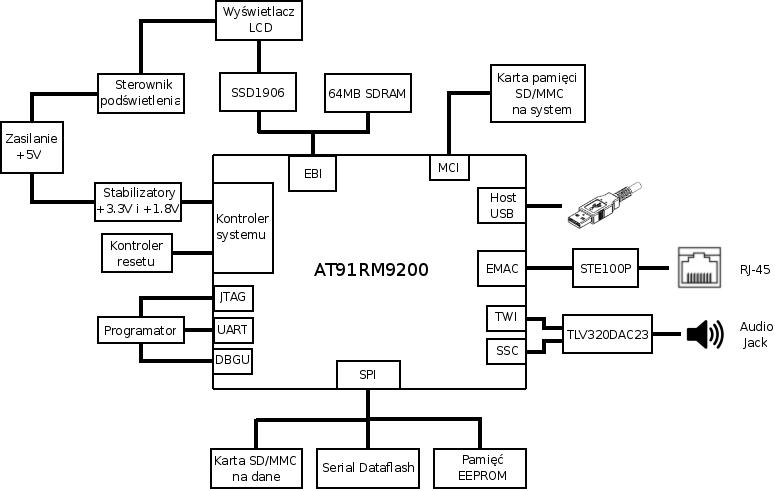
\includegraphics[scale=0.6]{img/schematic.jpg}
						\caption{Schemat blokowy projektu}
						\label{fig:block_schematic}
					\end{center}
				\end{figure}
				Rysunek \ref{fig:block_schematic} przedstawia schemat ideowy przykładowego rozwiązania platformy sprzętowej. Projekt zdecydowano wykonać w darmowej wersji programu do projektowania płytek drukowanych Eagle, jednak z powodu ograniczeń tej wersji (dozwolony maksymalny rozmiar pojedynczej płytki to 100mm*80mm) wystąpiła potrzeba podziału projektu na części opisane w punktach \ref{sec:main_board}, \ref{sec:ext_board} i \ref{sec:programator}. Podział taki spowodował uzyskanie projektu mniejszej wielkości oraz możliwość zmiany konfiguracji sprzętowej poprzez wymianę dodatkowej płytki PCB.\\
				Dwuwarstwowe płytki drukowane zostały wykonane w firmie Merkar z Katowic.\\
				Schematy ideowe, projekt PCB oraz zdjęcia wykonanego układu znajdują się w dodatku \ref{app:gotowy_projekt}.
			\subsection{Główna płytka sprzętowa}
				\label{sec:main_board}
				\subsubsection{Opis}
					Podstawowa część projektu jest w stanie samodzielnie obsługiwać system operacyjny Linux. W jej skład wchodzą:
					\begin{itemize}
						\item Mikroprocesor AT91RM9200
						\item Zasilanie układu oraz kontroler resetu
					\item 64MB pamięci SDRAM
						\item Złącze karty pamięci SD/MMC przeznaczonej na system operacyjny
						\item Sterownik warstwy fizycznej Ethernetu oraz gniazdko RJ-45
						\item Pamięć Serial Dataflash przechowująca programy uruchomieniowe
						\item Złącza dla programatora oraz dodatkowej płytki drukowanej
					\end{itemize}
					Za pomocą dwóch 40-pinowych złączy szpilkowych zostały wyprowadzone linie zasilania +3.3V i +5V oraz 54 linie ogólnego użytku, w tym magistrala EBI (External Bus Interface), TWI (Two Wire Interface), SPI (Serial Peripheral Interface), SSC (Synchronous Serial Controller).\\
				\subsubsection{Uwagi}
					\label{sec:uwagi}
					Podczas projektowania tej części platformy należało zwracać uwagę na wymienione poniżej zagadnienia.
					\begin{itemize}
						\item Do zasilania projektu użyto zasilacza impulsowego +5V/2.5A. Na wejściu zastosowano bezpiecznik 1.5A, diodę zabezpieczającą oraz serię kondensatorów elektrolitycznych i tantalowych.\\
						Ponieważ do działania układu jest dodatkowo konieczne napięcie +3.3V i +1.8V, zastosowano stabilizatory LM3940IMP-3.3 o maksymalnym obciążeniu prądowym 1A i LM1117-1.8 o obciążeniu 800mA.\\
						Napięcie +3.3V jest używane przez większość układów scalonych oraz transformator w gniazdku RJ-45. Do podświetlania wyświetlacza LCD jest potrzebne napięcie +5V, dlatego użyto bezpiecznika o dopuszczalnej wartości prądowej 1.5A.
						\item Ważne jest zapewnienie poprawnego startu mikrokontrolera dzięki podłączeniu pamięci Dataflash i zwarciu nóżki BMS mikrokontrolera poprzez opornik do napięcia zasilania. Po zresetowaniu mikrokontrolera zostanie uruchomiony program zawarty w pamięci ROM, który jest odpowiedzialny za przeszukanie kolejno pamięci Serial Dataflash podłączonej do portu SPI0, pamięci EEPROM dołączonej przez interfejs TWI oraz pamięci równoległej aktywowanej sygnałem NCS0, w celu znalezienia poprawnego wektora wskazującego na kod aplikacji. Jeśli taki wektor zostanie znaleziony to kod jest ładowany z danego układu do pamięci SRAM mikrokontrolera i stamtąd wykonywany. W przeciwnym razie nowy kod w postaci binarnej może zostać przesłany poprzez szeregowy interfejs DBGU za pomocą prokołu XModem lub łączem USB wykorzystując zaprojektowany przez Atmel protokół DFU (Device Firmware Upgrade). Po poprawnym ściągnięciu obrazu aplikacji do pamięci SRAM nastąpi wykonanie pierwszego rozkazu.\\
							W celu prawidłowego skonfigurowania portu szeregowego lub USB należy użyć rezonatora kwarcowego o jednej z wartości wskazanych w dokumentacji AT91RM9200 (np. 18.432MHz).
						\item Jako zewnętrzną pamięć SDRAM użyto dwóch kości o pojemności 32MB każda i szerokości słowa 16 bit. Aby uzyskać częstotliwość pracy magistrali powyżej 60MHz (przy takiej szybkości pracy linie używane do przesyłu danych zachowują się jak linie długie) należało zwracać szczególną uwagę na mogące wystąpić następujące problemy.
							\begin{itemize}
								\item Układy pamięci umieścić możliwie jak najbliżej procesora, aby skrócić czas propagacji sygnału. W projekcie udało się uzyskać minimalną długość linii ok. 20mm.
								\item Wszystkie ścieżki między procesorem a pamięcią powinny mieć jak najbardziej zbliżoną do siebie długość aby wyrównać czas propagacji sygnałów i impedancję linii. Z powodu braku miejsca na dwuwarstwowej płytce drukowanej wyrównanie długości nie było w pełni możliwe - uzyskano wartości rzędu 20-30mm.
							\end{itemize}
						\item Gniazda szpilkowe używane do połączenia z dodatkową płytką drukowaną powinny wyprowadzać jak najwięcej użytecznych linii sygnałowych oraz linie napięcia zasilania +3.3V i +5V.
					\end{itemize}
			\subsection{Dodatkowa płytka sprzętowa}
				\label{sec:ext_board}
				Na przykładowej dodatkowej płytce drukowanej znajdują się wymienione układy:
				\begin{itemize}
					\item Kontroler wyświetlacza LCD SSD1906, sterownik podświetlenia TPS61040 i złącza ZIF do podłączenia panelu TFT LQ043T3DX02.
					\item Przetwornik audio cyfrowo-analogowy TLV320DAC23 i gniazdo Jack 3.5mm dla słuchawek lub głośników aktywnych.
					\item Gniazdo na karty pamięci MicroSD do przechowywania danych użytkownika.
				\end{itemize}
				Podczas projektowania tej części platformy należało zwracać uwagę głównie na dostosowanie wymiarów w celu podłączenia do podstawowej płytki sprzętowej. Płytki są umieszczane jedna na drugiej i łączone za pomocą gniazda szpilkowego zatem żadne wystające elementy nie mogą znajdować się w tych samych rejonach. Dodatkowo istotne było właściwe ustawienie gniazda na taśmę wyświetlacza LCD.
			\subsection{Programator}
				\label{sec:programator}
				Aby zaoszczędzić miejsce na głównej płytce wchodzącej w skład projektu, zdecydowano że układy scalone, złącza, oraz pozostałe elementy używane tylko podczas programowania lub debuggowania układu będą znajdować się na osobnej płytce drukowanej dołączanej za pomocą 16-sygnałowego przewodu do transmisji danych. Programator zawiera zatem złącze do interfejsu JTAG, port szeregowy UART oraz port do debuggowania układu DBGU. Schemat ideowy programatora oraz projekt płytki drukowanej znajdują się na rysunku \ref{fig:programator} w dodatku \ref{app:gotowy_projekt}.
			\subsection{Lutowanie}
				Założeniem projektu było, aby był on możliwy do zlutowania bez potrzeby użycia zaawansowanego sprzętu. Do lutowania większości elementów wykorzystano zwykłą stację lutowniczą, jednak elementy o rozstawie nóżek 0.5mm (m.in. mikrokontroler AT91RM9200) przylutowano za pomocą stacji na gorące powietrze.
			
			\subsection{Problemy sprzętowe}
				W trakcie i po zlutowaniu projektu okazało się że wystąpiło kilka problemów:
				\begin{itemize}
					\item W projekcie płytki drukowanej zastosowano złe obudowy niektórych kondensatorów ceramicznych i rezonatora kwarcowego 32.768kHz.
					\item Po pierwszym uruchomieniu przepalił się bezpiecznik na wejściu układu. Po jego wymianie na bezpiecznik wielokrotny problem dalej występował - zauważono że jeden z kondensatorów tantalowych został wlutowany odwrotnie co powodowało duży pobór prądu przez układ.
					\item Podczas próby skomunikowania z układem poprzez JTAG okazało się że rozlutowane są nóżki procesora odpowiedzialne za przesył danych do programatora oraz źle przylutowany został przycisk resetujący układ przez co procesor był ciągle w stanie resetu. Po poprawieniu tych błędów komunikacja powiodła się.
					\item W projekcie programatora zastosowano zły schemat złącza DB-9 używanego do szeregowego przesyłu danych.
					\item Użyto złego schematu gniazda RJ-45 używanego przez port Ethernet co spowodowało niemożliwość używania sieci w projekcie.
					\item Ponieważ najpierw zaprojektowana i wykonana została podstawowa część platformy, podczas tworzenia dodatkowej płytki sprzętowej okazało się, że należy poprawić kilka elementów na głównej płytce PCB:
						\begin{itemize}
							\item Zapomniano o wyprowadzeniu napięcia zasilania +5V.
							\item Przydatny okazał się sygnał PCK0, który stanowi programowalny przez mikrokontroler sygnał zegarowy. Jest on używany przez układ SSD1906.
							\item W pierwotnej wersji projektu nie uwzględniono, że płytki znajdujące się w niedużej odległości jedna nad drugą, zawierają wystające elementy, takie jak kondensatory ceramiczne i złącza. Główna płytka sprzętowa została nieznacznie poprawiona pod tym względem.
						\end{itemize}
				\end{itemize}
				Wszystkie znalezione błędy zostały pomyślnie poprawione w ostatecznej wersji projektu.



%------------------------------------------------------------------------------------
% CZĘŚĆ PROGRAMOWA
%------------------------------------------------------------------------------------

	\chapter{Część programowa}
		\section{Wprowadzenie}
			Posiadając działającą platformę sprzętową można przejść do części programowej projektu, na którą składa się:
			\begin{itemize}
				\item Zapoznanie się ze sposobami programowej komunikacji, w tym samego programowania jak i debuggowania układu.
				\item Uruchomienie programu inicjalizującego (ang. bootloader), odpowiedzialnego za poprawne skonfigurowanie najważniejszych urządzeń sprzętowych zawartych w projekcie a następnie uruchomienie jądra systemu Linux.
				\item Konfiguracja i kompilacja linuksowego kernela.
				\item Utworzenie głównego systemu plików.
				\item Napisanie sterowników dla pozostałych potrzebnych urządzeń.
			\end{itemize}
			Dopiero na etapie programowania ujawnia się większość błędów sprzętowych zaistniałych w fazie projektowania platformy.
		\section{Programowanie układu}
		
			\subsection{OpenOCD}
				Aby połączyć się z układem mikroprocesorowym za pomocą złącza JTAG należy zastosować specjalne oprogramowanie, które pozwoli na przetworzenie poleceń użytkownika, wydawanych za pośrednictwem komputera PC, na odpowiednie polecenia protokołu JTAG.\\
				Jedną z takich aplikacji jest Open On-Chip Debugger\cite{website:openocd}, który działa na zasadzie serwera uruchamianego w tle i oczekującego na polecenia użytkownika.
				\subsubsection{Instalacja}
					Stabilną wersję OpenOCD można pobrać ze strony domowej projektu, jednak wersja 0.2.0 nie współdziałała poprawnie z zastosowanym w tej pracy układem sprzętowym JTAG. W związku z tym użyto działającej wersji numer 1679 dostępnej pod kontrolą źródeł SVN na stronie twórców.\\
					Aby skompilować i zainstalować aplikację należy doinstalować sterowniki odpowiednie dla obsługi sprzętowej używanego programatora JTAG. Na systemie operacyjnym Debian wystarczy, mając uprawnienia administratora, wydać komendę:\\
					\texttt{apt-get install libftdi1 libftdi-dev libusb-dev}\\
					W celu ściągnięcia i zainstalowania samej aplikacji należy wykonać ciąg następujących poleceń:\\
					\texttt{svn checkout -r 1679 svn://svn.berlios.de/openocd/trunk} - spowoduje pobranie z SVN-a odpowiedniej wersji OpenOCD\\
					\texttt{./bootstrap} - wstępna konfiguracja\\
					\texttt{./configure ----enable-maintainer-mode ----enable-ft2232\_libftdi ----prefix=/usr} - konfiguracja aplikacji; dołączenie biblioteki LibFTDI i ustawienie katalogu gdzie ma zostać zainstalowana na /usr\\
					\texttt{make \&\& make install} - kompilacja i instalacja\\
					Po poprawnym wykonaniu powyższych komend powinniśmy móc uruchomić oprogramowanie poprzez wykonanie polecenia \texttt{openocd}
					
				\subsubsection{Konfiguracja}
					Możliwe jest podanie opcji konfiguracyjnych bezpośrednio przy uruchomieniu OpenOCD lub zastosowanie plików konfiguracyjnych. Zgodnie z zaleceniami twórców, istotny jest podział konfiguracji na części istotne dla zastosowanego interfejsu służącego do programowania, używanego procesora oraz ustawień dodatkowych układów np. zewnętrznej pamięci SDRAM używanej w projekcie. W związku z tym ustawienia zostały podzielone na 4 części:
					\begin{itemize}
						\item{\texttt{openocd.cfg}}\\
							Główny plik konfiguracyjny definiujący m.in. używane porty.
							\begin{lstlisting}[basicstyle={\footnotesize\ttfamily}]
# Main configuration file
telnet_port 4444
gdb_port 3333
gdb_memory_map enable
gdb_flash_program enable
init
reset halt
							\end{lstlisting}
						\item{\texttt{interface/turtelizer.cfg}}\\
							Ustawienia interfejsu sprzętowego służącego do programowania.\\
							Opcja \texttt{jtag\_khz} służy do ustawiania szybkości interfejsu, lecz powinna być zmieniana dopiero po osiągnięciu odpowiedniej szybkości pracy mikroprocesora.
							\begin{lstlisting}[basicstyle={\footnotesize\ttfamily}]
# Configuration file for programming interface
interface ft2232
ft2232_device_desc "Turtelizer JTAG/RS232 Adapter"
ft2232_layout turtelizer2
ft2232_vid_pid 0x0403 0xbdc8			
jtag_khz 8
jtag_nsrst_delay 200
jtag_ntrst_delay 200
							\end{lstlisting}
						\item{\texttt{target/at91rm9200.cfg}}\\
							Opcje specyficzne dla zastosowanego mikroprocesora.
							\begin{lstlisting}[basicstyle={\footnotesize\ttfamily}]
# Configuration file for AT91RM9200 microprocessor
reset_config srst_only srst_pulls_trst

if { [info exists CHIPNAME] } {
   set  _CHIPNAME $CHIPNAME
} else {
   set  _CHIPNAME at91rm9200
}
if { [info exists ENDIAN] } {
   set  _ENDIAN $ENDIAN
} else {
   set  _ENDIAN little
}
if { [info exists CPUTAPID ] } {
   set _CPUTAPID $CPUTAPID
} else {
   set _CPUTAPID 0x05b0203f
}
# Never allow the following!
if { $_CPUTAPID == 0x15b0203f } {
   puts "-------------------------------------------------"
   puts "- ERR: TapID 0x15b0203f is wrong for at91rm9200 -"
   puts "- ERR: The board has a JTAG select jumper       -"
   puts "-------------------------------------------------"
}

jtag newtap $_CHIPNAME cpu -irlen 4 -ircapture 0x1 -irmask 0xf 
   -expected-id $_CPUTAPID

# Create the GDB Target.
set _TARGETNAME [format "%s.cpu" $_CHIPNAME]
target create $_TARGETNAME arm920t -endian $_ENDIAN -chain-position 
   $_TARGETNAME 
# AT91RM9200 has a 16K block of sram @ 0x0020.0000
$_TARGETNAME configure -work-area-virt 0x00200000 -work-area-phys 
   0x00200000 -work-area-size 0x4000 -work-area-backup 1
							\end{lstlisting}
						\item{\texttt{board/at91rm9200\_lab.cfg}}\\
							Dodatkowy plik który może zawierać komendy używane do ustawienia szybkości pracy mikroprocesora, konfiguracji odpowiednich układów wewnętrznych, pamięci SDRAM itp.
					\end{itemize}
				\subsubsection{Uruchamianie}
					W celu uruchomienia demona OpenOCD należy wywołać poniższą komendę, podając nazwy używanych plików konfiguracyjnych:\\
					\texttt{openocd -f openocd.cfg -f interface/turtelizer.cfg -f target/at91rm9200.cfg}\\
					Możliwe jest wtedy podłączenie się np. przez program telnet na odpowiedni port (\texttt{telnet localhost 4444}) i wykonanie przykładowych poleceń:
					\begin{itemize}
						\item\texttt{mdb <address>} - przeczytaj bajt spod podanego adresu
						\item\texttt{mwb <address> <value>} - zapisz bajt pod podany adres
						\item\texttt{reset} - resetuje mikroprocesor
						\item\texttt{halt} - zatrzymuje pracę mikroprocesora
						\item\texttt{resume} - wznawia pracę mikroprocesora
						\item\texttt{reg} - wyświetla lub ustawia zawartość rejestru, np. \texttt{reg pc 0} zeruje licznik rozkazów
						\item\texttt{bp <address> <length>} - ustawia breakpoint pod podanym adresem, <length> to długość rozkazu obsługiwana przez mikroprocesor
						\item\texttt{load\_image <file> <adress>} - załadowanie pliku binarnego pod wskazany adres
						\item\texttt{arm920t cache\_info} - informacja o pamięci Cache zastosowanej w rdzeniu ARM920T
						\item\texttt{help} - pełny spis poleceń
					\end{itemize}
				
			\subsection{Debug Unit (DBGU)}
				Debug Unit jest sprzętowym interfejsem mikrokontrolera, który pozwala na szeregowe przesyłanie danych pomiędzy programowanym układem a komputerem PC. Za pomocą jednostki DBGU można w całości zaprogramować platformę, bez potrzeby stosowania interfejsu JTAG.\\
				Aby komputer klasy PC mógł się poprawnie komunikować z mikrokontrolerem należy użyć szeregowego kabla typu null-modem oraz programu takiego jak HyperTerminal (Windows) lub minicom (Linux) i zastosować następujące parametry transmisji:\\
				\texttt{szybkość transmisji: 115200,\\liczba bitów danych: 8,\\bit parzystości:brak,\\bity stopu: 1}\\
				Po uruchomieniu platformy, na ekranie terminala (np. minicom) powinien pojawiać się znak 'C' zachęcający do rozpoczęcia transmisji danych. Niezaprogramowany mikrokontroler oczekuje w ten sposób na przesłanie kodu programu poprzez protokół XModem. Po otrzymaniu kodu binarnego zostaje on skopiowany do wewnętrznej pamięci SRAM, a następnie stamtąd uruchomiony.\\
				Bardziej szczegółowy opis postępowania podczas programowania znajduje się w sekcji \ref{sec:bootloader2nd}.
			\subsection{Środowisko do kompilowania}
				W celu skompilowania kodu źródłowego dla procesora o architekturze ARM należy użyć kompilatora skrośnego (ang. cross compiler). Kompilator taki jest uruchamiany na standardowym komputerze PC, ale zamiast kompilować kod do rozkazów np. procesora x86, potrafi kompilować i optymalizować programy dla architektury ARM. Oczywiście posiadając działający system oparty o mikroprocesor z rodziny ARM, można na nim zainstalować natywny kompilator i przeprowadzać kompilację do właściwej postaci, jednak zazwyczaj, z uwagi na dużą częstotliwość pracy najnowszych procesorów w zwykłych komputerach PC, szybciej i prościej jest przeprowadzić kompilację z użyciem kompilatora skrośnego.\\
				Podczas wyboru odpowiedniego kompilatora, nie zawsze najlepszym wyjściem jest pobranie najnowszych dostępnych wersji - należy zwrócić uwagę na kompatybilność kompilatora z dodatkowymi bibliotekami i aplikacjami takimi jak np. linker ld i debugger gdb. Kompilator używany do kompilacji programów dla innej architektury można zbudować samemu, jednak najlepiej zastosować stabilne i przetestowane środowisko (tzw. toolchain), które zostało już skompilowane dla danej architektury i posiada spełnione wszystkie wymagane zależności.\\
				W projekcie zastosowano toolchain pobrany ze strony \cite{website:gnuarm}, w którego skład wchodzi kompilator gcc-4.0.2-c-c++, dodatkowe aplikacje binarne binutils-2.16.1, oraz biblioteka C przeznaczona dla systemów wbudowanych newlib-1.14.0.

			\subsection{Eclipse}
				Podczas pisania oprogramowania, warto jest zastosować efektywne środowisko programistyczne, które może znacznie ułatwić proces tworzenia części programowej projektu.\\
				Jedną z popularniejszych aplikacji tego typu jest środowisko Eclipse, które pozwala na pisanie i kompilowanie oprogramowania w języku C, a także po odpowiedniej konfiguracji jego testowanie i debuggowanie na docelowej platformie dzięki zastosowaniu interfejsu JTAG. Szczegółowy opis konfiguracji został przedstawiony na stronie projektu YAGARTO\cite{website:yagarto}.
				
		\section{Bootloader}
			Bootloader, czyli pierwszy program uruchamiany po zresetowaniu mikrokontrolera, jest odpowiedzialny za zainicjalizowanie podstawowej funkcjonalności platformy, a następnie uruchomienie jądra systemu Linux. Mikrokontroler AT91RM9200 posiada wbudowany program inicjalizujący pierwszego poziomu, którego działanie zostało opisane w sekcji \ref{sec:uwagi}.\\
			Ponieważ program załadowany z Serial Dataflasha do pamięci SRAM może zajmować co najwyżej 16kB (w tym oprócz samego kodu należy uwzględnić obszar pamięci potrzebny na dane użytkownika) jego funkcjonalność jest znacznie ograniczona. Bardzo trudnym lub niewykonalnym zadaniem jest aby w tak niewielkiej ilości pamięci zmieścić aplikację, która będzie odpowiedzialna za skonfigurowanie pamięci SDRAM, odczytanie kernela z karty pamięci lub sieci i uruchomienie go. Dlatego zdecydowano się że program zawarty w pamięci ROM pobierze z pamięci Serial Dataflash i uruchomi bootloader drugiego poziomu (nazwany LAB Bootloader), którego zadaniem będzie konfiguracja pamięci SDRAM i wczytanie do niej głównego programu inicjalizującego. Dopiero główny bootloader, posiadający znacznie bardziej zaawansowaną funkcjonalność, zajmie się uruchomieniem jądra systemu operacyjnego Linux.\\
			Obydwa programy inicjalizujące są zapisane w pamięci Serial Dataflash (w projekcie użyto układu AT45DB041D o pojemności 512kB), ich rozmieszczenie zostało przedstawione na rysunku \ref{fig:bootloader_map}.
			\begin{figure}[]
				\begin{center}
					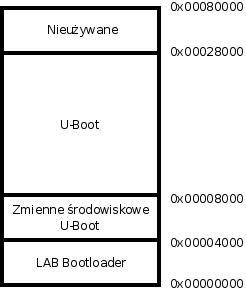
\includegraphics[scale=0.6]{img/bootloader_map.jpg}
					\caption{Zawartość pamięci Serial Dataflash}
					\label{fig:bootloader_map}
				\end{center}
			\end{figure}
			\subsection{Bootloader inicjalizujący}
				\label{sec:bootloader2nd}
				Jako bootloader drugiego poziomu (LAB Bootloader), czyli pierwszą aplikację której kod źródłowy jest dostępny dla użytkownika, zdecydowano się użyć stworzony przez firmę Atmel projekt RomBoot dla zestawu AT91RM9200DK\cite{website:arm_booting}. Kod został przeportowany dla kompilatora gcc zamiast ADS (ARM Developer Suite) a następnie nieznacznie uproszczony i dostosowany do potrzeb platformy sprzętowej. Zadaniem tego programu jest wykonanie następujących operacji:
				\begin{enumerate}
					\item Inicjalizacja wektorów przerwań i konfiguracja stosów dla różnych trybów pracy mikrokontrolera.
					\item Inicjalizacja kontrolera przerwań.
					\item Ustawienie poprawnej szybkości pracy procesora.
					\item Skonfigurowanie pamięci synchronicznej SDRAM.
					\item Zapoczątkowanie komunikacji poprzez port do debuggowania układu DBGU.
					\item Wyczyszczenie pamięci cache, ustawienie poprawnego trybu pracy układu, zezwolenie na przerwania.
					\item Inicjalizacja pamięci Serial Dataflash.
				\end{enumerate}
				Po pomyślnym wykonaniu powyższych czynności mikrokontroler automatycznie wystartuje główny program inicjalizujący po upływie określonego czasu (domyślnie 0.5 sekundy) lub będzie czekał na polecenia użytkownika. Obecna wersja aplikacji umożliwia wykonanie następujących poleceń:
				\begin{itemize}
					\item Pobranie danych poprzez port szeregowy pod wskazany adres pamięci Serial Dataflash.
					\item Przeczytanie zawartości pamięci SDRAM pod podanym adresem.
					\item Przeczytanie zawartości pamięci Serial Dataflash pod podanym adresem.
					\item Wystartowanie głównego bootloadera.
					\item Wyczyszczenie obszaru pamięci Dataflash zajmowanego przez podstawowy program inicjalizujący.
					\item Informacja o pamięci i bootloaderze.
				\end{itemize}
				Skompilowany i zoptymalizowany kod tego bootloadera zajmuje ok. 11kB. Rozmiar ten można jeszcze zmniejszyć ponieważ mikrokontroler AT91RM9200 umożliwia poprzez tzw. Embedded Software Services wykorzystanie funkcji które znajdują się w pamięci ROM i są używane przez bootloader pierwszego poziomu.\\
				Aby wgrać program inicjalizujący do pamięci Serial Dataflash należy połączyć platformę z komputerem PC za pomocą portu szeregowego DBGU, uruchomić skonfigurowaną aplikację terminala (np. minicom), a następnie zresetować mikrokontroler. Na ekranie terminala powinien zacząć się pojawiać znak 'C' informujący o możliwości zainicjalizowania transmisji danych. Po wybraniu odpowiedniej opcji rozpocznie się przesyłanie kodu binarnego bootloadera do pamięci SRAM mikroprocesora. Po zakończeniu transmisji użytkownik powinien zobaczyć menu programu inicjalizującego, a po jego wstępnym przetestowaniu można zapisać kod aplikacji do pamięci Serial Dataflash (wybór pierwszej opcji w menu). Użytkownik nigdy nie powinien zapisywać niedostatecznie sprawdzonego kodu bootloadera inicjalizującego w pamięci Dataflash - przed zapisaniem nowej wersji oprogramowania najlepiej wykasować starą zawartość pamięci, tak aby nowy kod mógł być najpierw przetestowany z poziomu pamięci SRAM.
				
			\subsection{Bootloader główny}
				Po analizie dostępnych rozwiązań, zdecydowano że jako główny bootloader zostanie użyty projekt U-Boot autorstwa Wolfganga Denka\cite{website:uboot}. Wybrany projekt został w znacznej mierze oparty na źródłach systemu operacyjnego Linux oraz posiada wsparcie dla mikrokontrolera AT91RM9200.\\
				Po pobraniu z internetu i poprawnym skompilowaniu za pomocą polecenia \texttt{make} przystąpiono do dostosowywania aplikacji do potrzeb docelowej platformy sprzętowej. W tym celu do katalogu \texttt{board/atmel/lab\_at91rm9200} skopiowano zawartość przykładowego projektu zawartego w \texttt{board/atmel/at91rm9200dk} i w dalszej kolejności wykonano następujące czynności:
				\begin{enumerate}
					\item Zmodyfikowano nazwę głównego pliku \texttt{at91rm9200dk.c} na \texttt{lab\_at91rm9200.c} i wszystkie nazwy oraz ścieżki w pliku \texttt{Makefile}.
					\item W pliku źródłowym \texttt{lab\_at91rm9200.c} usunięto funkcje odpowiedzialne za konfigurację pamięci NAND oraz zmieniono funkcję inicjalizującą interfejs sieciowy.
					\item W pliku \texttt{partition.c} zmieniono konfigurację zawartości pamięci Serial Dataflash (p. rys. \ref{fig:bootloader_map}).
					\item Do katalogu \texttt{cpu/arm920t/at91rm9200/}, który zawiera pliki źródłowe specyficzne dla zastosowanego mikrokontrolera skopiowano brakujące pliki:
						\begin{itemize}
							\item \texttt{atmel\_mci.c} - funkcje do obsługi interfejsu MCI
							\item \texttt{atmel\_mci.h} - plik nagłówkowy używany przez funkcje obsługujące MCI
							\item \texttt{ste100p.c} - funkcje do obsługi warstwy fizycznej interfejsu sieciowego
							\item \texttt{ste100p.h} - plik nagłówkowy używany przez powyższy plik źródłowy
						\end{itemize}
					\item W pliku \texttt{Makefile} w katalogu \texttt{cpu/arm920t/at91rm9200/} dodano wpisy dla plików obiektowych \texttt{atmel\_mci.o} i \texttt{ste100p.o}.
					\item Zmieniono pliki \texttt{drivers/mtd/dataflash.c} i \texttt{include/dataflash.h} pod kątem zastosowanego układu pamięci Serial Dataflash AT45DB041D.
					\item Dodano plik \texttt{include/asm-arm/arch-at91rm9200/mmc.h}.
					\item W pliku \texttt{include/configs/lab\_at91rm9200.h} utworzonym na podstawie przykładowego pliku konfiguracyjnego zmodyfikowano wartości takie jak szybkość pracy mikroprocesora, ilość dostępnej pamięci SDRAM oraz opcje dostępne w menu U-Boot.
					\item Dodano wpis dla platformy \texttt{lab\_at91rm9200} w głównym pliku \texttt{Makefile} projektu U-Boot oraz zmieniono ścieżkę dostępu do używanego kompilatora.
				\end{enumerate}
				Skompilowany kod w postaci binarnej umieszczono pod adresem 0x00008000 w pamięci Serial Dataflash za pomocą opcji dostępnej w bootloaderze inicjalizującym.\\
				\subsubsection{Uruchamianie}
				Pierwsze próby uruchomienia nie powiodły się - po zdebuggowania z użyciem JTAG-u okazało się że procesor wykonuje skok pod zły adres w pamięci. Ponieważ U-Boot jest uruchamiany z poziomu pamięci SDRAM sugerowało to problemy z czasami dostępu. Zewnętrzna magistrala używana podczas dostępu do pamięci była taktowana zegarem o częstotliwości 60MHz, niestety obniżenie szybkości pracy nie poprawiło efektów działania procesora.\\
				W pewnym stopniu pomogło wyłączenie w procesorze pamięci cache dla instrukcji. Spowodowało to jednak kilkukrotne spowolnienie działania układu, ponieważ kolejne rozkazy dla procesora były za każdym razem pobierane z pamięci SDRAM.\\
				W dalszej kolejności postanowiono sprawdzić poprawność działania pamięci SDRAM podczas szybkiego czytania i zapisywania danych. Aby tego dokonać napisano prostą aplikację opartą o bootloader inicjalizujący, której zadaniem było przeprowadzenie szeregu testów opisanych w dalszej części pracy.
				\begin{itemize}
 					\item \textbf{test adresowy} - Ten test zapisuje unikalną wartość w każdej komórce pamięci. Przykładowo moży to być adres tej komórki. Po zapisaniu dane są odczytywane i sprawdzane. 
					\item \textbf{maszerujący wzorzec} - Algorytm czyści zawartość pamięci, następnie odczytuje zawartość pierwszej komórki i zapisuje do niej wartość 1. Ta procedura odczytu i zapisu jest powtarzana dla wszystkich lokacji w pamięci. W tym momencie cała pamięć powinna być zapełniona liczbami 1. Kolejnym etapem testu jest poruszanie się od końca pamięci, odczyt kolejnych komórek i zamiana ich zawartości na 0. Po osiągnięciu początku pamięci test jest powtarzany z użyciem dopełnionych wartości.
					\item \textbf{galopujący wzorzec} - Test sprawdzający niepowtarzalność adresów i inne funkcjonalne błędy w pamięci, jak również niektóre dynamiczne przekłamania. Algorytm odwołuje się do każdej komórki pamięci używając po kolei każdego z pozostałych adresw jako miejsca, z którego nastąpi skok do sprawdzanej lokacji. Po wyczyszczeniu pamięci pierwsza komórka staje się adresem testowym - jest ona dopełniana i sprawdzana na zmianę z każdym z pozostałych adresów w całej pamięci. Każda kolejna komórka przyjmuje rolę testowej aż do momentu sprawdzenia całości.\\
					Z powodu dużej złożoności czasowej tego algorytmu, sprawdzono tylko kilka obszarów wielkości 1kB (czas wykonania takiego testu to ok. 40 minut).
				\end{itemize}
				Przeprowadzenie powyższych testów dla słów o długości 1, 2 i 4 bajtów nie wykazało żadnych błędów.\\
				Jak się okazało, problem stanowiła zbyt duża różnica w czasie dostępu do wbudowanej pamięci cache a zewnętrznej pamięci SDRAM. Rdzeń procesora taktowany zegarem 180MHz działał zbyt szybko podczas próby pobrania rozkazu z zewnętrznej pamięci, która korzystała z zegara o częstotliwości 60MHz. Po podwyższeniu tej wartości do 90MHz uruchomienie bootloadera U-Boot powiodło się.
		\section{Linux}
			W tym rozdziale zostanie opisany przebieg instalacji systemu operacyjnego Linux na docelowej platformie sprzętowej. Linux jest bardzo rozbudowanym systemem i daje użytkownikowi wiele możliwości konfiguracji, zarówno na etapie kompilacji jądra, jak i po uruchomieniu. Ponieważ celem tej pracy jest uruchomienie wbudowanej wersji Linuksa, na tym etapie należy zwrócić szczególną uwagę na wybór modułów wspieranych przez jądro, używaną dystrybucję (zestaw podstawowych aplikacji) oraz system plików.
			\subsection{Jądro systemu}
				\label{sec:linux_kernel}
				Jądro Linuksa jest w dużym stopniu zgodne ze standardami ANSI i POSIX, obsługuje wielozadaniowość, wielowątkowość, wielobieżność, pamięć wirtualną, biblioteki współdzielone, ładowanie na żądanie, współdzielony kod wykonywalny (ang. copy-on-write), dobre zarządzanie pamięcią i obsługę sieci TCP/IP.\\
				Poprzez zastosowanie modułowej budowy, można w trakcie konfiguracji zdecydować czy system powinien wspierać wybrane urządzenia, protokoły i inne funkcjonalności. Dzięki temu można dostosować kernel do konkretnych zadań, zmniejszyć ilość zajmowanej przez niego pamięci operacyjnej oraz zoptymalizować jego działanie.
				\subsubsection{Konfiguracja}
					W projekcie zdecydowano wykorzystać jądro systemu operacyjnego Linux w wersji 2.6.27.8 - jest to stabilne wydanie kernela, które zostało użyte w jednym z przykładowych projektów zawartych w dodatku \ref{app:przykladowe_projekty}, zatem posiadano pewność że ta wersja powinna działać.\\
					Spakowane archiwum zawierające źródła systemu operacyjnego należy pobrać ze strony internetowej \url{http://kernel.org/}, natomiast przydatne jest dodatkowo pobranie ze strony \url{http://maxim.org.za/at91_26.html} pliku z drobnymi poprawkami dla mikrokontrolera AT91RM9200 (plik jest dostępny w dołączonych materiałach). Aby go zastosować należy w głównym katalogu ze źródłami Linuksa wykonać polecenie:\\
					\texttt{zcat 2.6.27-at91.patch.gz | patch -p1}\\
					W dalszej kolejności należało wprowadzić modyfikacje niezbędne dla zastosowanej platformy sprzętowej m.in.
					\begin{itemize}
						\item Dodanie pliku \texttt{arch/arm/mach-at91/board-lab-at91rm9200.c} zawierającego funkcje używane podczas inicjalizacji płytki sprzętowej.
						\item Dołączenie w plikach \texttt{arch/arm/mach-at91/Kconfig} i \texttt{arch/arm/mach-at91/Makefile} nowych obiektów potrzebnych podczas konfiguracji i kompilacji.
						\item Dodanie obsługi warstwy fizycznej dla interfejsu sieciowego STE100P.
					\end{itemize}
					Powyższe poprawki są uwzględnione w pliku \texttt{linux-2.6.27.8-lab\_at91rm9200.patch.gz}.\\
					Po zastosowaniu wszystkich poprawek można przystąpić do wyboru konkretnych opcji konfiguracyjnych kernela - aby w tym celu skorzystać z pomocy graficznego narzędzia, należy wykonać polecenie \texttt{make ARCH=arm xconfig}.\\
					Uruchomiona w ten sposób aplikacja, zależnie od wybranej architektury sprzętowej procesora, dzieli strukturę kernela na kilkanaście kategorii. Opis ważniejszych z nich wraz z objaśnieniem wyboru modułów został przedstawiony poniżej. Niektóre funkcjonalności można zbudować jako moduły możliwe do załadowania w razie wystąpienia takiej potrzeby - jeśli system operacyjny nie będzie ich potrzebował będzie zajmował mniej miejsca w pamięci i działał szybciej. Jednakże w systemie wbudowanym zazwyczaj znana jest ostateczna konfiguracja i zadania jakie ma wykonywać platforma, zatem możliwe jest wbudowanie wszystkich wymaganych elementów w samo jądro.
					\begin{itemize}
						\item \textit{\textbf{General setup}} - Ogólne ustawienia kernela, domyślne ustawienia są poprawne.
							\begin{itemize}
								\item \textbf{Optimize for size} - Jeśli użytkownikowi zależy na rozmiarze zbudowanego obrazu jądra powinien włączyć tą opcję - spowoduje to przekazanie do kompilatora gcc flagi -Os zamiast -O2.
							\end{itemize}
						\item \textit{\textbf{Enable loadable module support}} - Pozwala na zastosowanie ładowalnych modułów.
							\begin{itemize}
								\item \textbf{Module unloading} - Pozwala na usuwanie modułów z przestrzeni kernela.
							\end{itemize}
						\item \textit{\textbf{System Type}} - Opcje specyficzne dla użytego mikrokontrolera.
							\begin{itemize}
								\item \textbf{ARM System Type} - Należy wybrać opcję Atmel AT91.
								\item \textbf{Support ARM920T processor} - Wsparcie dla rdzenia ARM920T zastosowanego w mikrokontrolerze AT91RM9200.
								\item \textbf{Disable I-cache / D-cache} - Włączenie pamięci cache na instrukcje i dane, powoduje znaczne przyspieszenie działania procesora.
								\item \textbf{Atmel AT91 System-on-Chip}
									\begin{itemize}
										\item \texttt{Atmel AT91 processor} - Należy wybrać AT91RM9200.
										\item \texttt{Linux ARM Board} - Jedna spośród dostępnych platform sprzętowych (ta pozycja pojawi się jeśli użytkownik zastosował poprawkę opisaną we wcześniejszej części tej sekcji).
										\item \texttt{Programmable clocks} - Aby używać jednego z programowalnych zegarów PCK0..3 należy zaznaczyć tą opcję - w omawianym projekcie linia PCK0 jest używana przez sterownik wyświetlacza LCD.
										\item \texttt{Select a UART for early kernel messages} - Port szeregowy wybrany do wyświetlania powiadomień na konsolę to DBGU.
									\end{itemize}
							\end{itemize}
						\item \textit{\textbf{Kernel features}}
							\begin{itemize}
								\item \textbf{Use the ARM EABI to compile the kernel} - EABI (Embedded Application Binary Interface) to zestaw reguł używanych we współpracy między aplikacjami i bibliotekami. Włączenie tej opcji powinno spowodować przyspieszenie działania systemu, jednak wymagane jest aby wszystkie aplikacje również były skompilowane z obsługą EABI.
							\end{itemize}
						\item \textit{\textbf{Boot options}} - Opcje ważne przy starcie Linuksa.
							\begin{itemize}
								\item \textbf{Default kernel command string} - Parametry przekazywane do jądra podczas ładowania głównego systemu plików. Przykład:\\
								\texttt{mem=64M console=ttyS0,115200 rootfstype=ext2 root=/dev/mmcblk0p2 rootdelay=4 init=/sbin/init}
							\end{itemize}
						\item \textit{\textbf{Networking support}} - Umożliwia użycie rozmaitych protokołów sieciowych, dla zbudowanej platformy sprzętowej ważne jest włączenie obsługi stosu TCP/IP oraz ew. modułów filtrujących pakiety (firewall Netfilter).
						\item \textit{\textbf{Device drivers}} - sterowniki wszystkich urządzeń wspieranych przez Linuksa
							\begin{itemize}
								\item \textbf{Memory Technology Device (MTD) support} - Jeśli używane są scalone układy pamięciowe takie jak np. Flash należy zwrócić uwagę na dostępne opcje. Dla opisywanej platformy sprzętowej wystarczy zaznaczyć opcję \texttt{AT91RM9200 DataFlash AT45DBxxx (legacy driver)}.
								\item \textbf{Block devices} - Urządzenia blokowe.
									\begin{itemize}
										\item \texttt{RAM block device support} - Przydatne gdy użytkownik chce używać części pamięci RAM jako urządzenia blokowego przechowującego system plików.
									\end{itemize}
								\item \textbf{Misc devices} - Różne urządzenia.
									\begin{itemize}
										\item \texttt{Device driver for Atmel SSC peripheral} - Włączenie obsługi interfejsu SSC (Synchronous Serial Communication) używanego przez przetwornik Audio TLV320DAC23.
									\end{itemize}								
								\item \textbf{Network device support} - W tym menu należy wybrać wsparcie dla sterownika warstwy fizycznej \texttt{STE100P} oraz warstwy łącza danych (opcja \texttt{AT91RM9200 Ethernet support}). Jeśli używane są sieciowe urządzenia USB należy dodatkowo wybrać odpowiednią opcję.
								\item \textbf{Input device support} - Obsługa urządzeń wskazujących, w tym klawiatur i myszek.
								\item \textbf{Character devices} - Wsparcie dla urządzeń znakowych.
									\begin{itemize}
										\item \texttt{Legacy (BSD) PTY support} - Włączenie tej opcji powodowało częste błędy podczas startowania systemu Linux. Nowe aplikacji linuksowe nie powinny używać pseudoterminali BSD, dlatego bezpieczne jest wyłączenie tej opcji.
										\item \texttt{SPI driver (legacy) for AT91RM9200 processors} - W czasie działania systemu protokół SPI będzie używany tylko do obsługi dodatkowej karty pamięci SD/MMC.
										\item \texttt{Serial drivers} - W celu debuggowania układu ważne jest zezwolenie na używanie portu szeregowego jako konsoli poprzez opcję \texttt{Support for console on AT91/AT32 serial port}.
									\end{itemize}
								\item \textbf{SPI support} - W tym menu należy wybrać właściwy kontroler dla protokołu SPI (\texttt{Atmel SPI Controller}).
								\item \textbf{Watchdog timer support} - Jeśli użytkownik chce używać układu resetującego działanie procesora w przypadku bezczynności (w celu wykrywania błędów w aplikacjach) powinien włączyć tą opcję.
								% TODO: framebuffer?
								\item \textbf{USB support} - Wsparcie dla rozmaitych urządzeń USB.
								\item \textbf{MMC/SD card support} - Obsługa protokołów MMC i SD.
									\begin{itemize}
										\item \texttt{MMC block device driver} - Spowoduje skonfigurowanie czytnika kart pamięci jako urządzenia blokowego. Możliwe staje się wtedy korzystanie z systemu plików zawartego na karcie.
										\item \texttt{AT91 SD/MMC Card Interface support} - Wybranie interfejsy MCI firmy Atmel.
									\end{itemize}
								\item \textbf{Real time clock} - Umożliwia korzystanie z wbudowanego w AT91RM9200 zegara czasu rzeczywistego.
							\end{itemize}
						\item \textit{\textbf{File systems}} - Wybór głównego systemu plików został przedstawiony w sekcji \ref{sec:filesystem}. Użytkownik może w tym menu zaznaczyć dodatkowe systemy plików jako moduły, co spowoduje ich dynamiczne załadowanie w razie potrzeby.				
					\end{itemize}
					Po zapisaniu zostanie utworzony plik \texttt{.config} zawierający wszystkie wybrane opcje.
				\subsubsection{Kompilacja}
					W celu zbudowania nowego jądra systemu operacyjnego Linux należy wykonać serię wymienionych poniżej poleceń:
					\begin{itemize}
						\item \texttt{make ARCH=arm dep} - utworzenie wszystkich zależności
						\item \texttt{make ARCH=arm clean} - wyczyszczenie pozostałości po poprzednio budowanym kernelu
						\item \texttt{make ARCH=arm CROSS\_COMPILE=/opt/gnuarm-4.0.2/bin/arm-elf-} - skompilowanie jądra dla architektury ARM z użyciem podanego kompilatora skrośnego
						\item \texttt{make ARCH=arm CROSS\_COMPILE=/opt/gnuarm-4.0.2/bin/arm-elf- uImage} - \\utworzenie obrazu binarnego, który może zostać uruchomiony przez bootloader
					\end{itemize}
					Przed wykonaniem ostatniego kroku należy się upewnić, czy aplikacja \texttt{mkimage} zawarta w katalogu \texttt{tools} bootloadera U-Boot jest widoczna podczas budowania jądra (jeśli nie jest, należy dodać katalog \texttt{tools} do zmiennej środowiskowej \texttt{PATH}). Narzędzie \texttt{mkimage} służy do dodania niedużego nagłówka do zbudowanego obrazu, tak aby U-Boot wiedział spod jakiego adresu należy wystartować jądro systemu operacyjnego Linux.\\
					Po pomyślnym wykonaniu podanych poleceń w katalogu \texttt{arch/arm/boot/} źródeł Linuksa powinien znaleźć się plik \texttt{uImage} będący skompresowanym obrazem systemu operacyjnego (jego rozmiar dla wybranej konfiguracji to ok. 1MB).\\
					Dodatkowo, jeśli użytkownik wybrał kompilację niektórych funkcji jako modułów należy wykonać polecenia:
					\begin{itemize}
						\item \texttt{make ARCH=arm CROSS\_COMPILE=/opt/gnuarm-4.0.2/bin/arm-elf- modules}
						\item \texttt{make ARCH=arm CROSS\_COMPILE=/opt/gnuarm-4.0.2/bin/arm-elf- \\INSTALL\_MOD\_PATH=. modules\_install}
					\end{itemize}
					Odpowiednie pliki z rozszerzeniem \texttt{.ko}, zawierające skompilowane moduły linuksowe, będą znajdowały się w podkatalogu \texttt{lib/modules/2.6.27.8}. Aby działający system mógł je poprawnie załadować należy skopiować podany katalog do głównego katalogu w docelowym systemie plików, lub posiadając zamontowany system plików stosowany na platformie zmienić wartość zmiennej \texttt{INSTALL\_MOD\_PATH}.
			\subsection{Dystrybucja}
				Dystrybucja, czyli zestaw aplikacji i bibliotek tworzących razem z kernelem działający system operacyjny, podobnie jak samo jądro, w wersji dla systemów wbudowanych różni się nieznacznie od tych przeznaczonych dla komputerów biurkowych i serwerów. Różnica polega głównie na przemyślanym doborze wszystkich aplikacji, tak aby zaoszczędzić dostępne miejsce na nośnikach danych i w pamięci operacyjnej oraz zoptymalizować działanie. Aby idealnie dostosować system do danej platformy sprzętowej użytkownik może sam skompilować wszystkie wymagane programy, a następnie utworzyć strukturę głównego systemu plików, jednak takie podejście wymaga dużego nakładu pracy.\\
				Na rynku jest dostępnych wiele darmowych i komercyjnych rozwiązań, wśród których są standardowe dystrybucje (skompilowane na konkretną platformę sprzętową) oraz środowiska służące do konfigurowania i budowania dystrybucji.
				\subsubsection{MontaVista}
					Komercyjne rozwiązanie rozwijane przez firmę MontaVista Software, która ma duży wpływ na dodawanie nowych funkcjonalności i poprawek do jądra Linuksa. Oprogramowanie jest wykorzystywane m.in. w modułach GPS, przenośnych przyrządach medycznych i innych urządzeniach mobilnych.\\
					Dzięki wieloletnim pracom nad tą dystrybucją, twórcom udało się osiągnąć m.in.:
					\begin{itemize}
						\item Szybkie uruchomienie systemu
						\item Dynamiczne zarządzanie energią co pozwala na wydłużenie czasu pracy z użyciem baterii
						\item Obsługa żądań w czasie rzeczywistym
						\item System zajmuje niedużo pamięci
						\item Aplikacje wspierające wiele protokołów przesyłu danych
						\item Zaawansowane środowisko programistyczne MontaVista DevRocket
					\end{itemize}
				\subsubsection{Android}
					Zaawansowany system operacyjny tworzony przez firmę Google dla potrzeb urządzeń mobilnych. Spośród cech Androida warte wymienienia są:
					\begin{itemize}
						\item Wsparcie dla bibliotek 3D bazujących na OpenGL
						\item Baza danych SQLite
						\item Możliwość komunikacji poprzez GSM/EDGE, CDMA, UMTS, Bluetooth i Wi-Fi
						\item Maszyna wirtualna Javy
						\item Możliwość odtwarzania plików multimedialnych zapisanych w wielu popularnych formatach
						\item Android może obsługiwać m.in. aparaty fotograficzne, ekrany dotykowe, moduły GPS i akcelerometry
					\end{itemize}
					W chwili pisania tej pracy nie istniała wersja Androida przeznaczona dla mikrokontrolera AT91RM9200, jednak został pomyślnie stworzony wariant dla innego układu firmy Atmel - AT91SAM9261. Jest to bardzo rozbudowana dystrybucja - stworzona platforma sprzętowa nie jest w stanie wykorzystać znacznej większości dostępnych opcji.
				\subsubsection{OpenWRT}
					Dystrybucja, zawierająca menadżer pakietów \texttt{opkg}, wykorzystywana głównie przez urządzenia sieciowe m.in. routery WLAN firmy Linksys. Na jej podstawie utworzono kilka cieszących się dobrą opinią użytkowników systemów, takich jak HyperWRT i Tomato.\\
					Użycie OpenWRT dla potrzeb opisywanej platformy sprzętowej wymagałoby jednak samodzielnego kompilowania wszystkich programów, ponieważ nie istnieje wersja przeznaczona dla architektury ARM.
				\subsubsection{Emdebian}
					Oparte o popularny system operacyjny Debian środowisko dostarczające narzędzia do kompilowania aplikacji a następnie ich umieszczania w pakietach \texttt{.deb} oraz tworzenia wymaganego przez Linux głównego systemu plików. W archiwach Debiana znajduje się bardzo duża liczba aplikacji i bibliotek skompilowanych dla architektury ARM, a dzięki narzędziu \texttt{apt-get} możliwe jest ich instalowanie przy wykorzystaniu sieci Internet.\\
					Wadą tego systemu jest konieczność zainstalowania środowiska budującego na komputerze PC zawierającym system operacyjny Debian GNU/Linux.
				\subsubsection{OpenEmbedded}
					Środowisko służące do konfigurowania i budowania własnej dystrybucji. Jego zaletami są m.in.
					\begin{itemize}
						\item Wsparcie dla wielu architektur sprzętowych
						\item Zawiera narzędzia do kompilacji skrośnej
						\item OpenEmbedded można uruchomić na każdej dystrybucji Linuksa
						\item Pozwala na skompilowanie pakietów takich jak GTK+, Qt, X.org, Mono i Java
					\end{itemize}
					W skład projektu wchodzi zestaw skryptów BitBake, które zawierają ścieżkę URL z kodem źródłowym pakietu, jego zależności i opcje używane podczas kompilacji lub instalacji. Dodatkowo środowisko może zająć się skompilowaniem jądra Linuksa oraz utworzeniem głównego systemu plików, tworząc w ten sposób kompletny obraz partycji zawierającej gotowy do uruchomienia system operacyjny Linux.\\
					Na podstawie OpenEmbedded zostało opartych wiele dystrybucji m.in. MontaVista Linux 6 i \r{A}ngstr\"{o}m Linux.
				\subsubsection{Buildroot}
					Buildroot jest narzędziem podobnym do OpenEmbedded, jednak posiada graficzny konfigurator, który pozwala na łatwiejsze dostosowanie systemu do potrzeb użytkownika. W skład środowiska wchodzi zestaw skryptów Makefile oraz poprawek, które pozwalają na pobranie z sieci, skonfigurowanie i zbudowanie narzędzi do kompilacji skrośnej, jądra Linuksa, aplikacji i bibliotek, a następnie połączenie ich wszystkich w gotowy system plików.\\
					Najważniejszą cechą Buildroota jest to, że jako biblioteki języka C używa przeznaczonej dla systemów wbudowanych biblioteki $\mu$Clibc. W odróżnieniu od standardowej wersji tej biblioteki, czyli glibc, $\mu$Clibc zajmuje o wiele mniej miejsca i nie posiada zaimplementowanych rzadko używanych funkcji.\\
					Aby uruchomić aplikację konfiguracyjną należy wykonać polecenie \texttt{make menuconfig}. Oprócz wyboru odpowiedniej architektury sprzętowej i toolchaina wykorzystującego bibliotekę $\mu$Clibc, użytkownik powinien zająć się selekcją programów wchodzących w skład dystrybucji. Spośród ciekawszych aplikacji warte wymienienia są:
					\begin{itemize}
						\item \textbf{BusyBox} - Napisana z myślą o systemach wbudowanych aplikacja, która w pojedynczym pliku wykonywalnym mieści funkcjonalność wielu standardowych komend uniksowych takich jak np. \texttt{ls}, \texttt{find}, \texttt{grep}, \texttt{cat}, \texttt{ps}, \texttt{bash}, \texttt{vi}, \texttt{bzip2}.\\
							Poszczególne aplikacje zawarte w BusyBox są uruchamiane poprzez osobne dowiązania symboliczne do głównego pliku wykonywalnego.
						\item \textbf{SQLite} - Wydajny system zarządzania bazą danych SQL który bardzo dobrze nadaje się do systemów wbudowanych.
						\item \textbf{Dropbear} - Nieduża aplikacja serwera i klienta protokołu SSH 2 umożliwiającego bezpieczne połączenia sieciowe.
						\item \textbf{TFTPd} - Serwer obsługujący oparty o UDP uproszczony protokół przesyłu danych TFTP (Trivial File Transfer Protocol). Przydatny w momencie, gdy użytkownik chce szybko skopiować jakiś plik na docelową platformę.
						\item \textbf{Matchbox} - Popularny w systemach wbudowanych menadżer okien. Wymaga skonfigurowanego serwera X.
						\item \textbf{ipkg} - System zarządzania pakietami. Pozwala na pobranie z sieci i instalację dodatkowego oprogramowania.
						\item \textbf{microperl} - Okrojona wersja interpretera skryptów napisanych w języku Perl.
					\end{itemize}
					Buildroot umożliwia również pobranie z sieci i zbudowanie jądra systemu operacyjnego Linux - opis jak tego dokonać manualnie został przedstawiony w sekcji \ref{sec:linux_kernel}.\\
					Ostatnią ważną czynnością którą należy wykonać jest wybór odpowiedniego systemu plików z jakiego będzie korzystać zbudowana dystrybucja. Opis dostępnych opcji został przedstawiony w następnym podrozdziale.\\
					Po ustawieniu wszystkich opcji i zapisaniu konfiguracji użytkownik może wykonać polecenie \texttt{make}, co spowoduje rozpoczęcie kilkugodzinnego procesu pobierania wszystkich potrzebnych plików z sieci i ich kompilacji.
			\subsection{System plików}
				\label{sec:filesystem}
				Po uruchomieniu jądra systemu operacyjnego na tym etapie użytkownikowi ukaże się komunikat podobny do tego:\\
				\texttt{Kernel panic – not syncing: VFS: Unable to mount root fs on unknown-\\block(0,0)}\\
				Jest to informacja o tym, że kernel nie był w stanie zamontować głównego systemu plików, na którym powinny znajdować się wszystkie pliki wchodzące w skład dystrybucji.\\
				Podczas wyboru systemu plików najbardziej odpowiedniego dla zastosowania konkretnej platformy sprzętowej należy kierować się czynnikami takimi jak:
				\begin{itemize}
					\item \textbf{Zapis}\\
						Jeśli żadne dane nie muszą być aktualizowane lub zbierane na urządzeniu, system plików nie musi dawać możliwości zapisu danych. Możliwe jest jednak połączenie systemu plików tylko do zapisu z systemem takim jak UnionFS lub aufs, który umożliwia zapis zmienionych danych i uwzględnienie różnic przy ponownym zamontowaniu.
					\item \textbf{Trwałość danych}\\
						Specyfika niektórych urządzeń nie musi gwarantować zapisania danych po ponownym uruchomieniu - zmiany mogą być widoczne  tylko w pamięci operacyjnej.
					\item \textbf{Odporność na zanik zasilania}\\
						Niektóre systemy plików np. Ext2 mogą zostać zepsute i wymagać naprawy w momencie nagłego zaniku napięcia zasilania i ponownego uruchomienia urządzenia. Czasami ważne jest aby system pracujący np. w warunkach przemysłowych był w stanie działać bez interwencji użytkownika w momencie wystąpienia takiego zdarzenia.
					\item \textbf{Kompresja}\\
						Jeśli użytkownikowi zależy na ilości miejsca zajmowanego przez zamontowany system, powinien zastanowić się nad użyciem skompresowanego systemu plików. Potrzebne dane są rozkompresowywane w pamięci operacyjnej.
					%\item \textbf{Korzystanie z pamięci RAM}\\
					%	System plików może w całości lub częściowo znajdować się w pamięci operacyjnej urządzenia. Nie jest wtedy konieczne użycie trwałego nośnika danych - zawartość systemu plików może być np. pobrana z serwera sieciowego NFS.
				\end{itemize}
				Spośród wielu systemów plików, które mogą być obsługiwane przez jądro Linuksa, tylko kilka nadaje się do wykorzystania przez systemy wbudowane i mogą być utworzone za pomocą środowiska Buildroot. Poniżej zostaną przedstawione 4 z nich, natomiast w tabeli \ref{tab:fs_comparison} znajduje się krótkie podsumowanie ich właściwości.
				
				\begin{itemize}
					\item \textbf{CRAMFS} - Compressed ROM File System został zaprojektowany z myślą o prostocie i oszczędności miejsca. Każda strona pamięci jest skompresowana osobno za pomocą algorytmów z biblioteki \texttt{zlib}, natomiast dane opisujące rozmieszczenie plików nie są spakowane. CRAMFS nie umożliwia zapisu danych, zatem nie mają znaczenia takie właściwości jak trwałość danych oraz odporność na zaniki zasilania. Maksymalny rozmiar tego systemu plików to ok. 272MB.
					\item \textbf{JFFS2} - Journalling Flash File System został stworzony specjalnie dla układów pamięciowych Flash. Jest to system plików o strukturze loga. Podczas montowania, zawartość całego nośnika danych musi zostać przeskanowana w celu stworzenia struktury katalogów w pamięci RAM, co dla nośników o dużej pojemności może stanowić problem.
					\item \textbf{SquashFS} - System plików podobny do CRAMFS, jednak dzięki zastosowaniu algorytmu LZMA umożliwia na uzyskanie stopnia kompresji rzędu 25\%. Posiada kilka usprawnień oraz potrafi obsługiwać pliki o rozmiarach do 2\textasciicircum64 bajtów.
					\item \textbf{Ext2} - Jeden ze standardowych systemów plików używanych przez system operacyjny Linux. Dane są zapisywane na nośniku przy każdej zmianie, co przy ograniczonej liczbie cyklów zapisu na zastosowanej karcie pamięci jest wadą tego systemu. Dodatkowo system ten nie jest odporny na zaniki napięcia zasilania - wystąpienie takiej sytuacji może doprowadzić do trwałego uszkodzenia systemu.
				\end{itemize}
				\begin{table}[h]
					\extrarowheight=3pt
					\begin{tabularx}{\textwidth}{|c|X|X|X|X|X|}
						\hline \textbf{System plików} & \textbf{Zapis} & \textbf{Trwałość danych} & \textbf{Odporność na zanik zasilania} & \textbf{Kompresja} \\
						\hline \textbf{CRAMFS} & nie & - & - & tak \\
						\hline \textbf{JFFS2} & tak & tak & tak & tak \\
						\hline \textbf{SquashFS} & nie & - & - & tak \\
						\hline \textbf{Ext2} & tak & tak & nie & nie \\
						\hline
					\end{tabularx}
					\caption{Porównanie systemów plików}
					\label{tab:fs_comparison}
				\end{table}
				System plików JFFS2 wydaje się najbardziej odpowiedni dla zastosowania w systemie wbudowanym, jednak został on zaprojektowany z myślą o urządzeniach NAND i NOR Flash i pomimo tego że został napisany sterownik dla kart pamięci SD/MMC, nie jest on tak efektywny. Oprócz tego wykorzystanie tego systemu dla nośników danych o dużej pojemności spowodowałoby zużycie znacznej ilości pamięci operacyjnej platformy.\\
				Pomimo swoich wad, system plików Ext2 wydaje się dobrym kandydatem do przechowywania głównego katalogu używanego przez system operacyjny Linux. Ewentualnie można zastanowić się nad jednoczesnym wykorzystaniem kilku systemów plików, np. Ext2 do przechowywania plików konfiguracyjnych, SquashFS dla zainstalowanych aplikacji i bibliotek, natomiast TMPFS dla danych tymczasowych.\\
				W projekcie platformy zdecydowano się na przykładowy podział karty pamięci SD/MMC na dwie partycje przedstawiony na rysunku \ref{fig:sd_mmc}. Pierwsza partycja jest używana tylko przez U-Boot w celu wczytania jądra systemu operacyjnego Linux do pamięci operacyjnej.\\
				\begin{figure}[h!]
					\begin{center}
						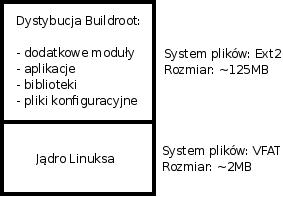
\includegraphics[scale=0.7]{img/sd_mmc.jpg}
						\caption{Podział karty pamięci SD/MMC o pojemności 128MB}
						\label{fig:sd_mmc}
					\end{center}
				\end{figure}\\			
				Po zbudowaniu Buildroota w katalogu \texttt{binaries} powinien znaleźć się obraz partycji Ext2 zawierającej główny katalog utworzonej dystrybucji. Aby nagrać obraz na utworzoną partycję należy wykonać polecenie:\\
				\texttt{dd if=rootfs.arm.ext2 of=/dev/sdb2 bs=512}\\
				gdzie \texttt{/dev/sdb2} to druga partycja karty pamięci SD/MMC.\\
				W dalszej kolejności należy wyedytować plik \texttt{/etc/fstab} aby ustawić prawidłowy punkt montowania głównej partycji docelowej dystrybucji. Przykładowa zawartość tego pliku została przedstawiona na poniższym listingu.
				\begin{lstlisting}[basicstyle={\footnotesize\ttfamily}]
# /etc/fstab: static file system information.
# <file system> <mount pt> <type> <options>               <dump> <pass>
/dev/mmcblk0p2  /          ext2   defaults,rw,noatime     0      1
proc            /proc      proc   defaults                0      0
devpts          /dev/pts   devpts defaults,gid=5,mode=620 0      0
tmpfs           /tmp       tmpfs  defaults                0      0
sysfs           /sys       sysfs  defaults                0      0	

				\end{lstlisting}
			\subsection{Uruchamianie}
				W celu uruchomienia systemu operacyjnego Linux na zbudowanej platformie sprzętowej podzielono kartę pamięci SD/MMC na partycje w sposób podany na rysunku \ref{fig:sd_mmc}. Po nagraniu jądra Linuksa i dystrybucji Buildroot podłączono napięcie zasilania co spowodowało wystartowanie przez mikrokontroler programu inicjalizującego LAB Bootloader. Po odczekaniu odpowiedniego czasu lub wybraniu odpowiedniej opcji został uruchomiony bootloader U-Boot.\\
				W momencie uruchamiania systemu operacyjnego Linux, procesor powinien znajdować się w takim stanie, jak gdyby został dopiero uruchomiony. W związku z tym ostatnią czynnością wykonywaną przez bootloader przed wystartowaniem Linuksa jest uruchomienie funkcji \texttt{cleanup\_before\_linux}, która jest odpowiedzialna za wyłączenie przerwań oraz pamięci cache dla instrukcji i danych. Szybkość pracy procesora oraz konfiguracja pamięci SDRAM i innych układów powinny zostać niezmienione.\\
				Aby zmusić U-Boot do wczytania jądra systemu operacyjnego Linux należy wykonać ciąg instrukcji przedstawionych poniżej (czynność tą można zautomatyzować poprzez ustawienie odpowiednich zmiennych środowiskowych i zapisanie ich w pamięci Serial Dataflash).
				\begin{enumerate}
					\item \texttt{mmcinit} - Inicjalizacja dostępnych kart pamięci SD/MMC.
					\item \texttt{fatls mmc 0} - Wyświetlenie zawartości pierwszej karty pamięci.
					\item \texttt{fatload mmc 0 0x21000000 uImage} - Wczytanie pliku binarnego \texttt{uImage}, zawierającego obraz kernela, z głównego katalogu pierwszej karty pamięci pod adres \texttt{0x21000000} pamięci operacyjnej platformy.
					\item \texttt{bootm 0x21000000} - Uruchomienie jądra systemu operacyjnego spod podanego adresu pamięci.
				\end{enumerate}
				Po wykonaniu powyższych czynności rozpocznie się wczytywanie obrazu Linuksa:
				\begin{lstlisting}[basicstyle={\footnotesize\ttfamily}]
## Booting kernel from Legacy Image at 21000000 ...                             
   Image Name:   Linux-2.6.27.8                                                 
   Image Type:   ARM Linux Kernel Image (uncompressed)                          
   Data Size:    1135352 Bytes =  1.1 MB                                        
   Load Address: 20008000                                                       
   Entry Point:  20008000                                                       
   Verifying Checksum ... OK                                                    
   Loading Kernel Image ... OK                                                  
OK                                                                              
                                                                                
Starting kernel ...                                                             
                                                                                
Uncompressing Linux................................................
.............
Linux version 2.6.27.8 (odi@debian) (gcc version 4.0.2) #41 Mon Oct 
12 22:56:209
CPU: ARM920T [41129200] revision 0 (ARMv4T), cr=c0006173                        
Machine: Linux ARM Board                                                        
Memory policy: ECC disabled, Data cache buffered                                
Clocks: CPU 179 MHz, master 89 MHz, main 18.432 MHz                             
CPU0: D VIVT write-back cache                                                   
CPU0: I cache: 16384 bytes, associativity 64, 32 byte lines, 8 sets             
CPU0: D cache: 16384 bytes, associativity 64, 32 byte lines, 8 sets             
Built 1 zonelists in Zone order, mobility grouping on.  Total pages: 
16256      
Kernel command line: mem=64M console=ttyS0,115200 rootfstype=ext2 
root=/dev/mmcblk0p2 rootdelay=3 init=/sbin/init
AT91: 96 gpio irqs in 3 banks                                                   
PID hash table entries: 256 (order: 8, 1024 bytes)                              
Console: colour dummy device 80x30                                              
console [ttyS0] enabled                                                         
Dentry cache hash table entries: 8192 (order: 3, 32768 bytes)                   
Inode-cache hash table entries: 4096 (order: 2, 16384 bytes)                    
Memory: 64MB = 64MB total                                                       
Memory: 62548KB available (2040K code, 180K data, 96K init)                     
Calibrating delay loop... 89.79 BogoMIPS (lpj=16384)                             
Mount-cache hash table entries: 512                                             
CPU: Testing write buffer coherency: ok                                         
net_namespace: 288 bytes                                                        
NET: Registered protocol family 16                                              
usbcore: registered new interface driver usbfs                                  
usbcore: registered new interface driver hub                                    
usbcore: registered new device driver usb                                       
NET: Registered protocol family 2                                               
IP route cache hash table entries: 1024 (order: 0, 4096 bytes)
TCP established hash table entries: 2048 (order: 2, 16384 bytes)
TCP bind hash table entries: 2048 (order: 1, 8192 bytes)
TCP: Hash tables configured (established 2048 bind 2048)
TCP reno registered
NET: Registered protocol family 1
NetWinder Floating Point Emulator V0.97 (double precision)
msgmni has been set to 122
io scheduler noop registered (default)
at91_spi: Baud rate set to 5616000
AT91 SPI driver loaded
atmel_usart.0: ttyS0 at MMIO 0xfefff200 (irq = 1) is a ATMEL_SERIAL
atmel_usart.1: ttyS1 at MMIO 0xfffc4000 (irq = 7) is a ATMEL_SERIAL
atmel_usart.2: ttyS2 at MMIO 0xfffc8000 (irq = 8) is a ATMEL_SERIAL
brd: module loaded
eth0: Link down.
eth0: AT91 ethernet at 0xfefbc000 int=24 10-HalfDuplex (00:25:73:01:23:45)
eth0: STE100P PHY
at91_ohci at91_ohci: AT91 OHCI
at91_ohci at91_ohci: new USB bus registered, assigned bus number 1
at91_ohci at91_ohci: irq 23, io mem 0x00300000
usb usb1: configuration #1 chosen from 1 choice
hub 1-0:1.0: USB hub found
hub 1-0:1.0: 1 port detected
usb usb1: New USB device found, idVendor=1d6b, idProduct=0001
usb usb1: New USB device strings: Mfr=3, Product=2, SerialNumber=1
usb usb1: Product: AT91 OHCI
usb usb1: Manufacturer: Linux 2.6.27.8 ohci_hcd
usb usb1: SerialNumber: at91
mice: PS/2 mouse device common for all mice
at91_rtc at91_rtc: rtc core: registered at91_rtc as rtc0
AT91 Real Time Clock driver.
AT91 Watchdog Timer enabled (5 seconds, nowayout)
usbcore: registered new interface driver usbhid
usbhid: v2.6:USB HID core driver
TCP cubic registered
NET: Registered protocol family 17
at91_rtc at91_rtc: setting system clock to 1998-01-01 00:00:27 UTC 
(883612827)
Waiting 3sec before mounting root device...
mmc0: new MMC card at address 0001
mmcblk0: mmc0:0001 128M   125440KiB 
 mmcblk0: p1 p2
EXT2-fs warning: mounting unchecked fs, running e2fsck is recommended
VFS: Mounted root (ext2 filesystem).
Freeing init memory: 96K
Populating /dev using udev: done
Initializing random number generator... read-only file system 
detected...done
Starting network...
ifup: interface lo already configured
Starting HPA's tftpd: done

Welcome to Linux ARM Board
lab login: root
Dec 31 17:00:48 login[258]: root login on 'ttyS0'
# 
				\end{lstlisting}
				
			\subsection{Dodatkowe moduły}
				\label{sec:linux_modules}
				Każdy z dodatkowych układów wchodzących w skład projektu, wymaga specjalizowanego modułu programowego umożliwiającego komunikację między rejestrami takiego układu, a warstwami systemu operacyjnego Linux. Dzięki zmodularyzowanej budowie Linuksa, w celu utworzenia kodu odpowiadającego za komunikację z niewspieranym jeszcze układem, w większości przypadków wystarczy napisać obsługę kilku funkcji odpowiadających za niskopoziomową komunikację (np. zapis i odczyt z rejestrów), natomiast resztą pracy zajmą się wyższe warstwy aplikacji odpowiadające za większą część funkcjonalności.\\
				W dostępnych źródłach systemu operacyjnego nie została zaimplementowana obsługa układów opisanych w trzech kolejnych podpunktach.
				
				\subsubsection{Ethernet}
					Aby móc korzystać z interfejsu sieciowego platformy, konieczna była implementacja obsługi sterownika wartwy fizycznej STE100P. W projekcie wykorzystano kod napisany przez Grzegorza Rajtara (p. załącznik \ref{app:przykladowe_projekty}).\\
					 Procesor komunikuje się z układem scalonym STE100P za pomocą interfejsu MII (Media Independent Interface), którego implementacja znajduje się w jądrze Linuksa, dlatego nie ma potrzeby zajmowania się obsługą wymiany danych pomiędzy obydwoma układami.\\
					 Sam moduł składa się z funkcji odpowiedzialnych za następujące działania:
					 \begin{itemize}
					 	\item inicjalizacja układu
					 	\item obsługa przerwań
					 	\item autonegocjacja parametrów transmisji
					 	\item zawieszenie i wznowienie pracy układu
					 \end{itemize}
					 Pozostałą funkcjonalnością niezbędną do korzystania z sieci Ethernet zajmują się wyższe warstwy aplikacyjne modelu ISO/OSI. Są one niezależne od zastosowanej konfiguracji sprzętowej oraz bardzo dobrze przetestowane.
				\subsubsection{Kontroler LCD}
					Jednym z założeń projektu była możliwość podłączenia kolorowego wyświetlacza LCD. Aby w znacznym stopniu odciążyć procesor od konieczności odświeżania obrazu zastosowano specjalizowany kontroler LCD - układ SSD1906 firmy Solomon, który dzięki odpowiedniej konfiguracji umożliwia podłączenie paneli STN, TFT i HR-TFT. Komunikuje się on z procesorem za pomocą magistrali równoległej, która jest używana również do komunikacji z pamięcią SDRAM platformy. Rejestry i 256kB wewnętrznej pamięci SRAM układu SSD1906 są widziane przez procesor pod adresem 0x40000000.\\
					Linuksowy moduł jądra, potrafiący obsłużyć sterownik wyświetlacza opiera się na idei tzw. bufora ramki (ang. framebuffer). Aplikacje wyświetlające obraz komunikują się z urządzeniem \texttt{/dev/fb0}, które jest zależne od niskopoziomowej implementacji sprzętowej sterownika, natomiast sam kontroler LCD jest widziany przez kernel i sterownik framebuffera jako obszar pamięci do którego można zapisać obraz.\\
					Zadania linuksowego modułu układu SSD1906 są następujące:
					\begin{itemize}
						\item inicjalizacja układu
						\item zarezerwowanie wymaganej przez moduł pamięci
						\item odczyt i zapis rejestrów
						\item ustawienie trybu pracy m.in. żądanej liczby kolorów
						\item zarządzanie rejestrami LUT (Look-Up Table)
						\item regulacja podświetlenia wyświetlacza
					\end{itemize}
					Dzięki zastosowaniu bufora ramki, możliwe jest wyświetlanie obrazu już podczas ładowania systemu Linux. Niektóre aplikacje i biblioteki linuksowe, takie jak odtwarzacz multimedialny MPlayer czy biblioteka SDL, potrafią korzystać bezpośrednio z framebuffera, bez potrzeby używania serwera graficznego X, co jest szczególnie przydatne w systemach wbudowanych.\\
					W momencie oddawania tej pracy, moduł kontrolera LCD został napisany lecz niedostatecznie przetestowany.
				\subsubsection{Sterownik Audio}
					Komunikacja z układem scalonym TLV320DAC23 odbywa się za pośrednictwem interfejsów TWI i SSC. Moduł tego sterownika powinien zajmować się głównie ustawianiem trybu pracy m.in. częstotliwości próbkowania, natomiast pozostała część pracy należy do systemu ALSA (Advanced Linux Sound Architecture), z którym komunikują się aplikacje użytkownika mogące odtwarzać dźwięk.\\
					W chwili oddawania tej pracy, programowy sterownik układu TLV320DAC23 nie został jeszcze zaimplementowany.
%		\section{Aplikacja demonstracyjna}
		
	\chapter{Podsumowanie}
		Wszystkie założenia postawione we wstępie pracy zostały w pełni zrealizowane.\\
		Okazało się, że przy znajomości podstaw elektroniki, techniki układów cyfrowych oraz konfiguracji i działania systemu operacyjnego Linux, możliwe jest wykonanie prostego urządzenia posiadającego możliwości zbliżone do tych, spotykanych w dostępnych na rynku urządzeniach przenośnych.\\
		Podczas realizacji pracy natrafiono na szereg problemów, wymagających zapoznania się m.in. z zasadami projektowania obwodów drukowanych działających dla częstotliwości wyższych niż 60MHz, procesem uruchamiania mikroprocesora ARM oraz niskopoziomowej konfiguracji systemu operacyjnego Linux.\\
		Dzięki podziałowi platformy sprzętowej na dwie części - główną, posiadającą podstawową funkcjonalność, oraz dodatkową, umożliwiającą przykładowe podłączenie wyświetlacza oraz przetwornika audio - możliwa jest stosunkowo łatwa zmiana konfiguracji sprzętowej.Przykładowym zastosowaniem stworzonego projektu jest proste urządzenie multimedialne, będące w stanie odtwarzać dźwięk i obraz, którego sterowanie odbywać się może za pośrednictwem łącza Ethernet lub klawiatury USB. Kolejnym celem podczas prac nad projektem może być utworzenie interfejsu sieciowego uruchamianego na prostym serwerze HTTP, umożliwienie przechowywania plików na dodatkowej karcie pamięci lub dołączanym dysku USB oraz zastosowanie wyświetlacza LCD z panelem dotykowym.\\
		Systemy wbudowane oparte na Linuksie cieszą się coraz większym powodzeniem, ze względu na koszty wprowadzenia na rynek, otwartość kodu źródłowego oraz stabilność dostępnych aplikacji. Po skonfigurowaniu systemu operacyjnego do własnych potrzeb, użytkownik może od razu korzystać z bardzo rozbudowanej funkcjonalności, bez potrzeby pisania dodatkowego kodu.
		
	\bibliographystyle{plain}
	\bibliography{bibliography}
	
	%\cite{ldd3}
	%\cite{building_embedded}
	
	
	\appendix
	
	\chapter{Gotowy projekt}
	\label{app:gotowy_projekt}
		\begin{figure}[h!]
			\begin{center}
				\label{fig:cpu_sch}
				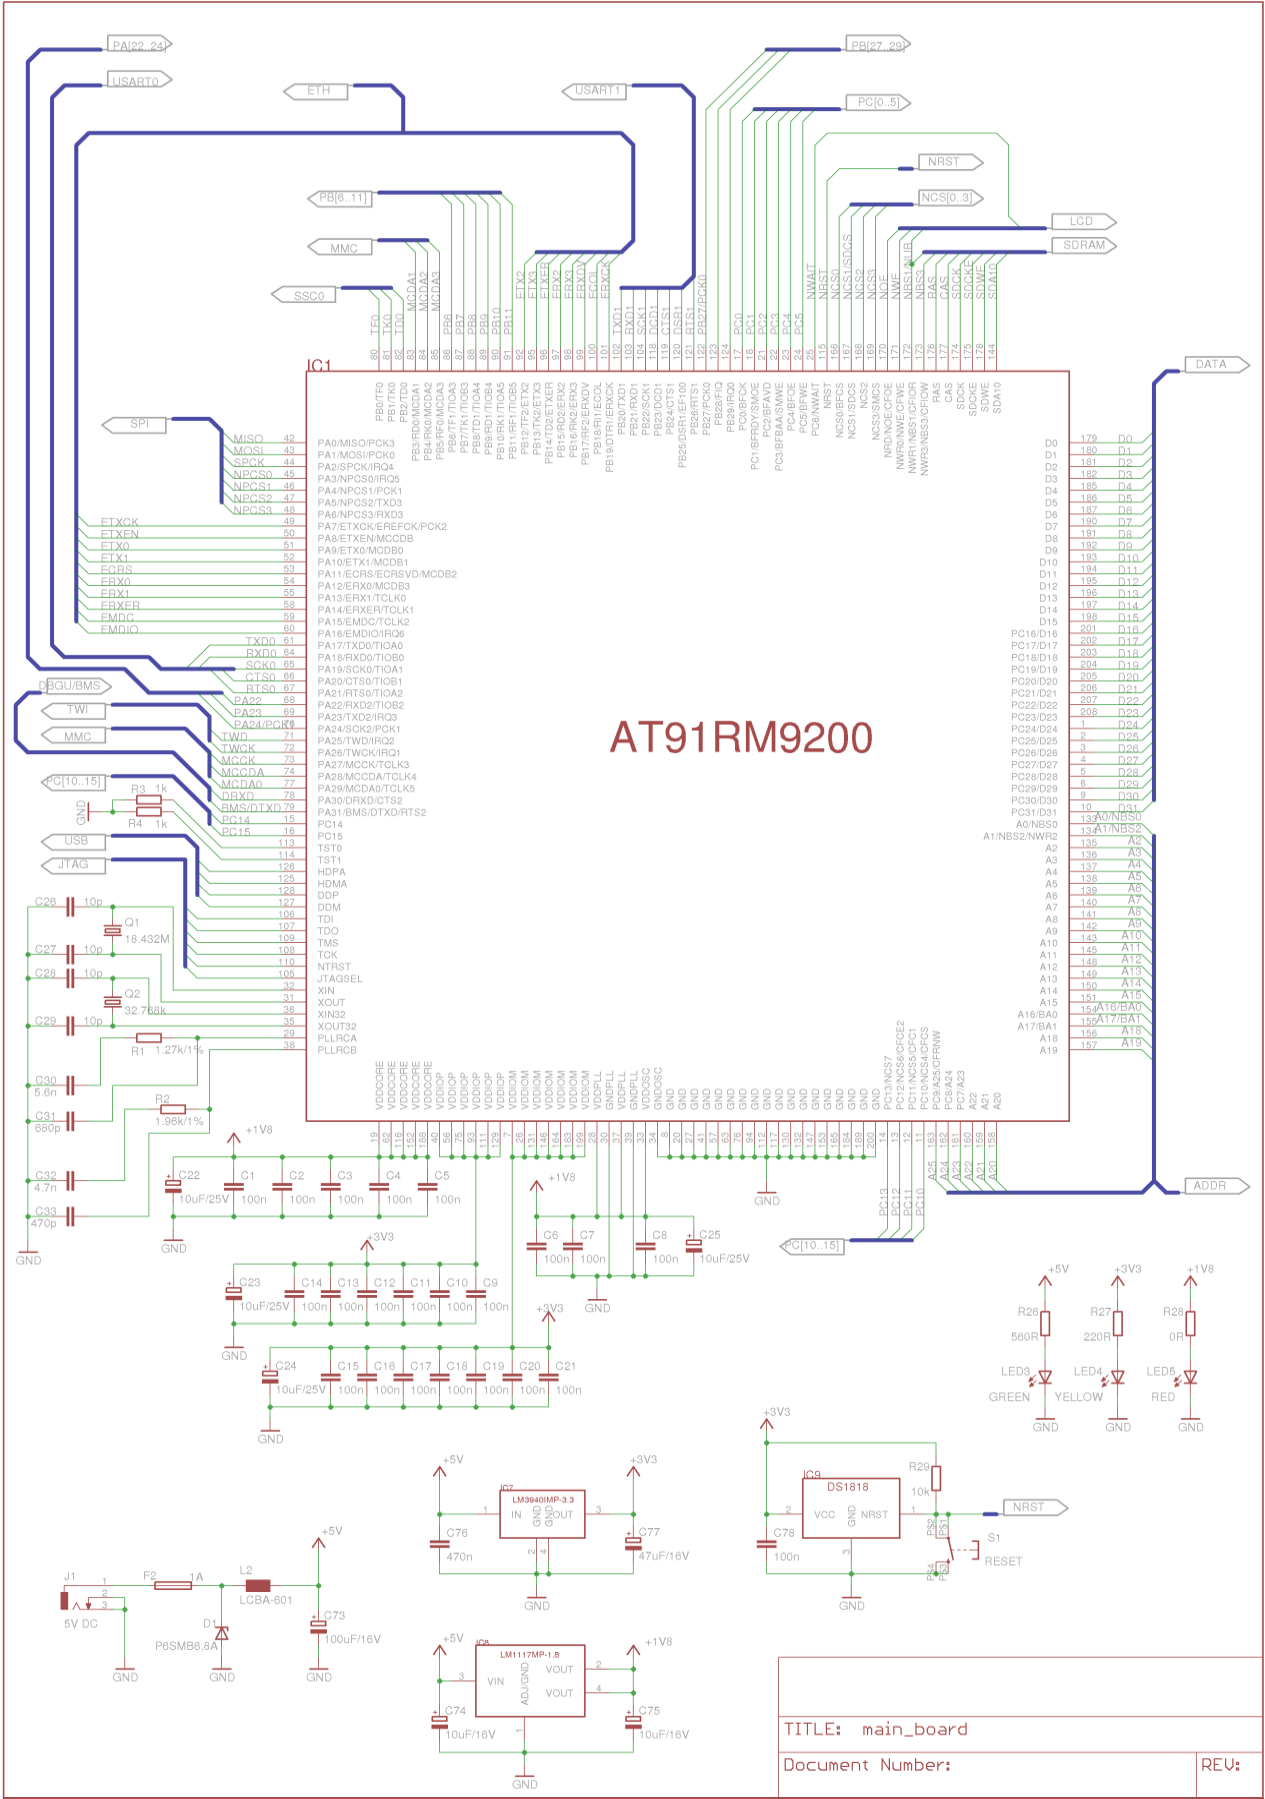
\includegraphics[scale=1.0]{img/cpu_sch.png}
				\caption{Schemat podłączenia mikrokontrolera}
			\end{center}
		\end{figure}
		
		\begin{figure}[h!]
			\begin{center}
				\label{fig:main_sch}
				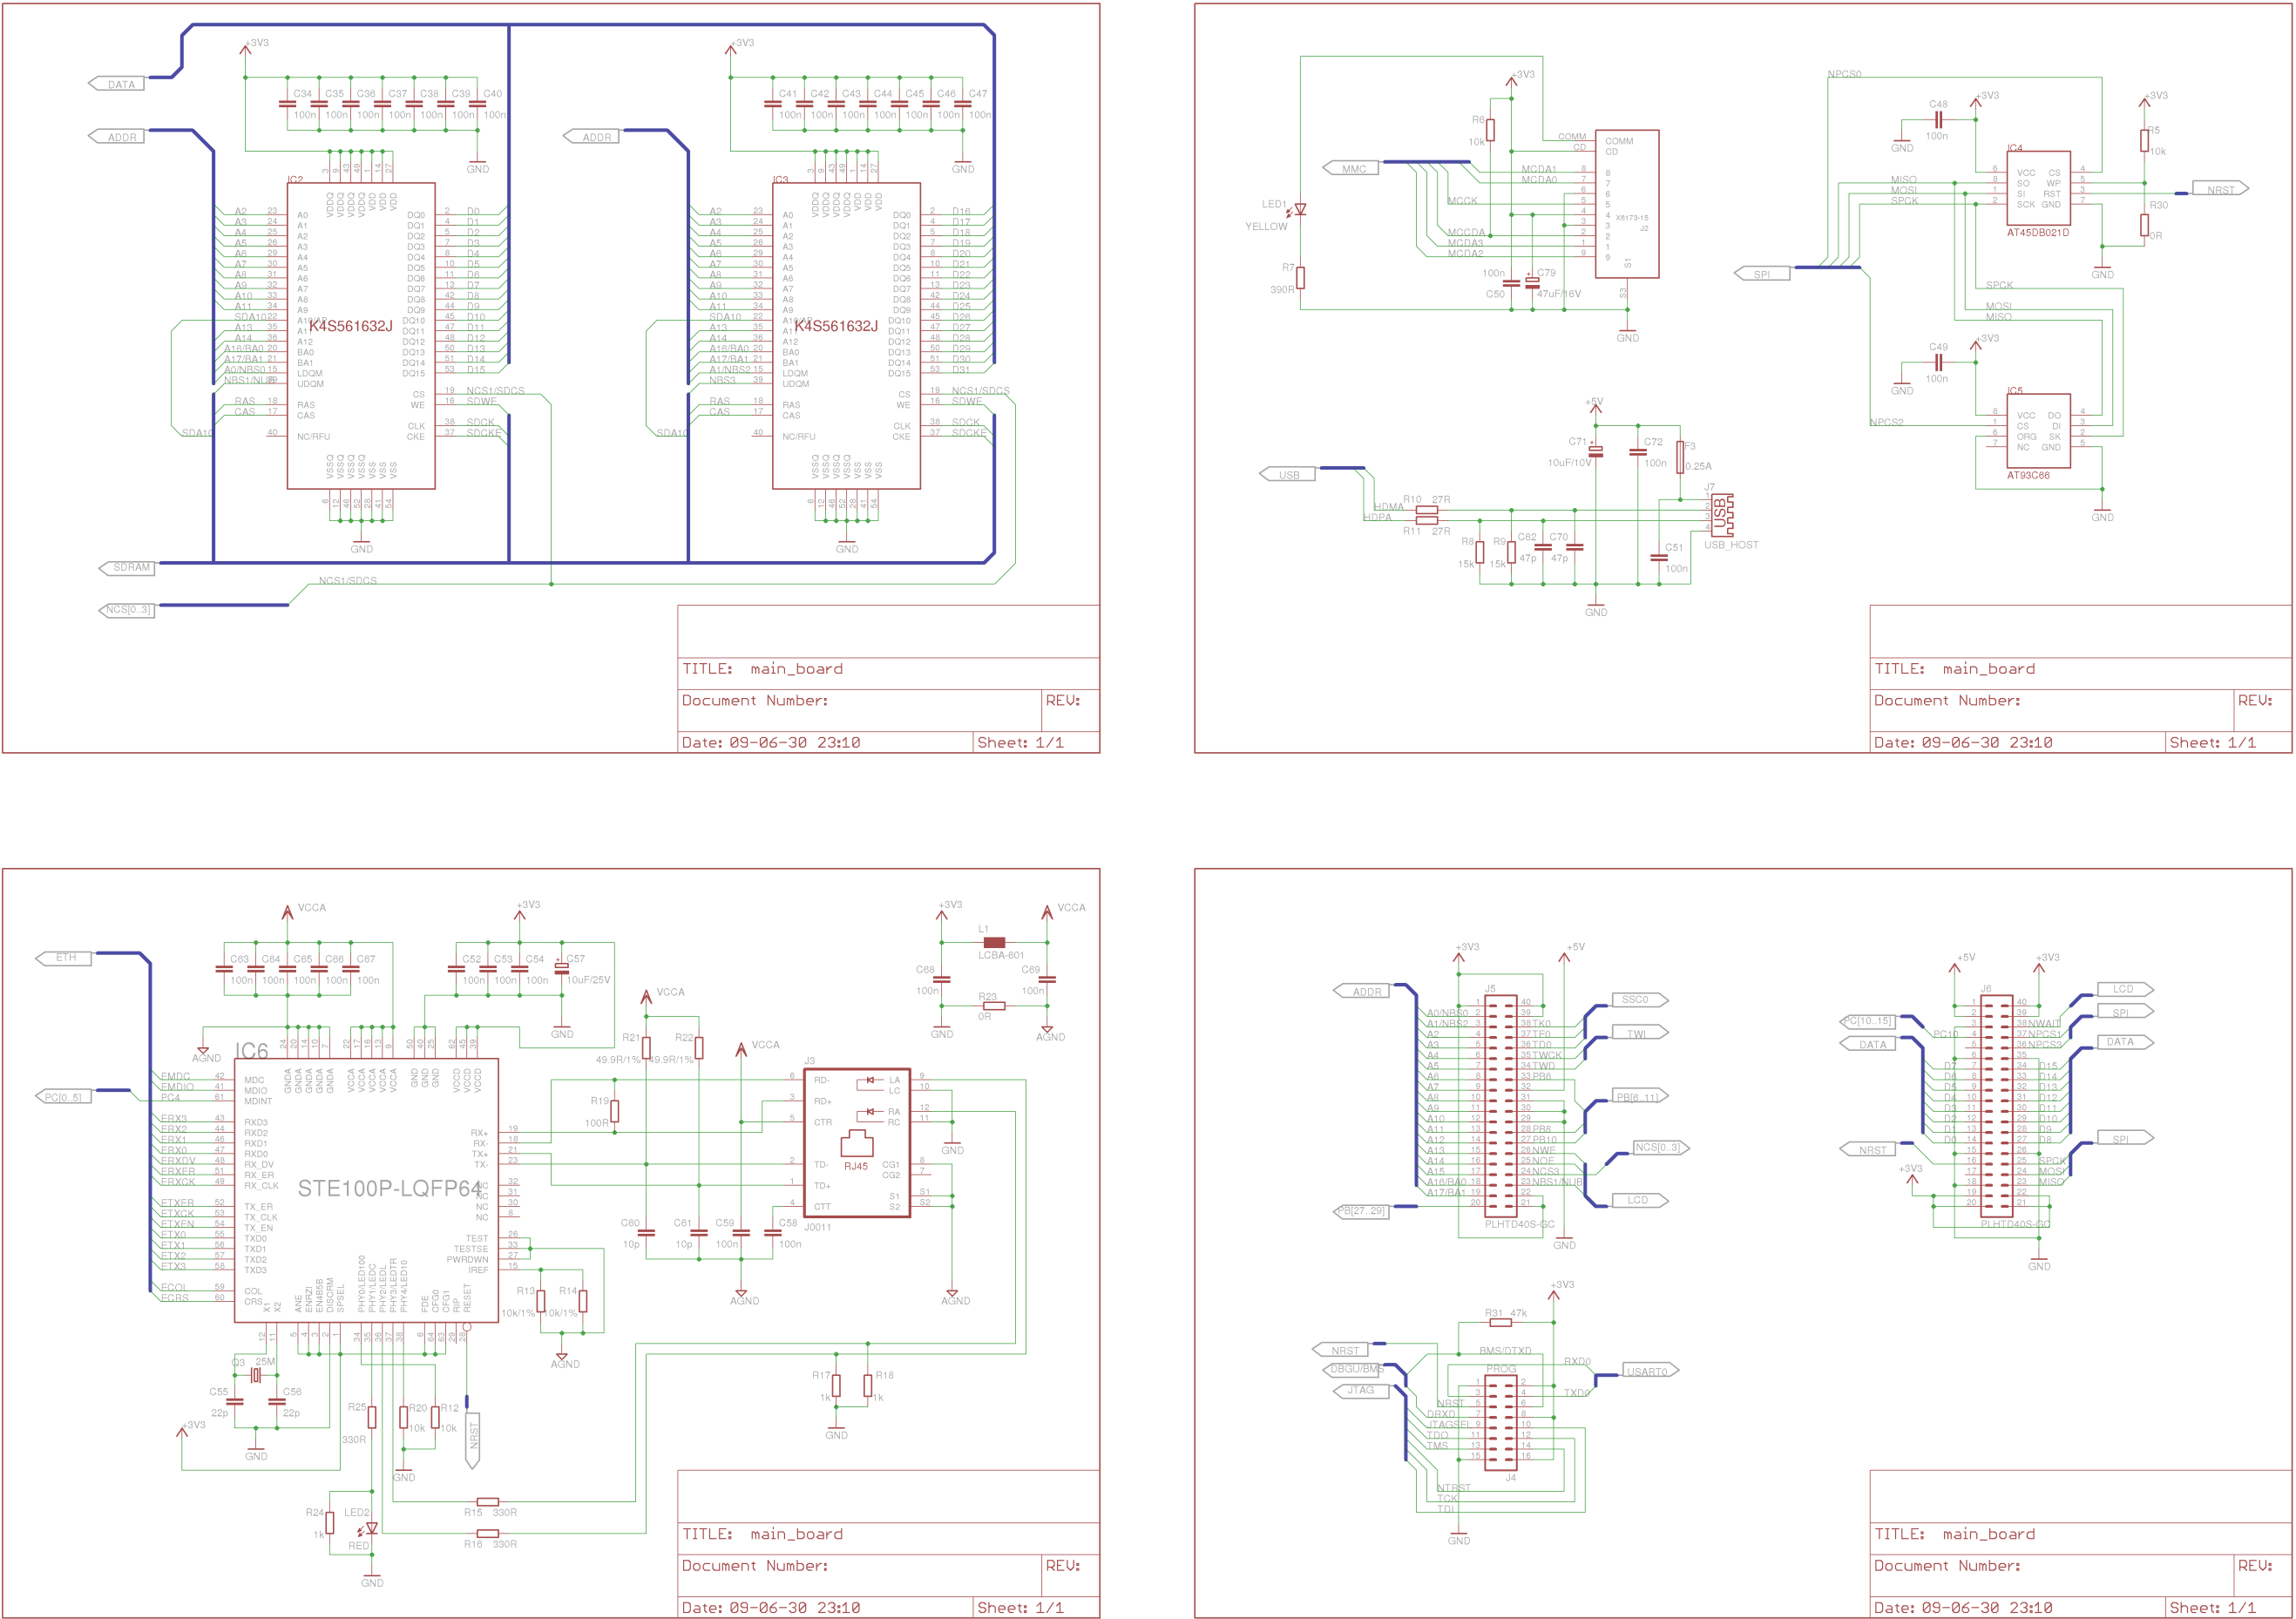
\includegraphics[scale=1.0,angle=90]{img/main_sch.png}
				\caption{Schemat podłączenia dodatkowych układów do głównej części projektu}
			\end{center}
		\end{figure}
		
		\begin{figure}[]
			\begin{center}
				\label{fig:ext_sch_lcd}
				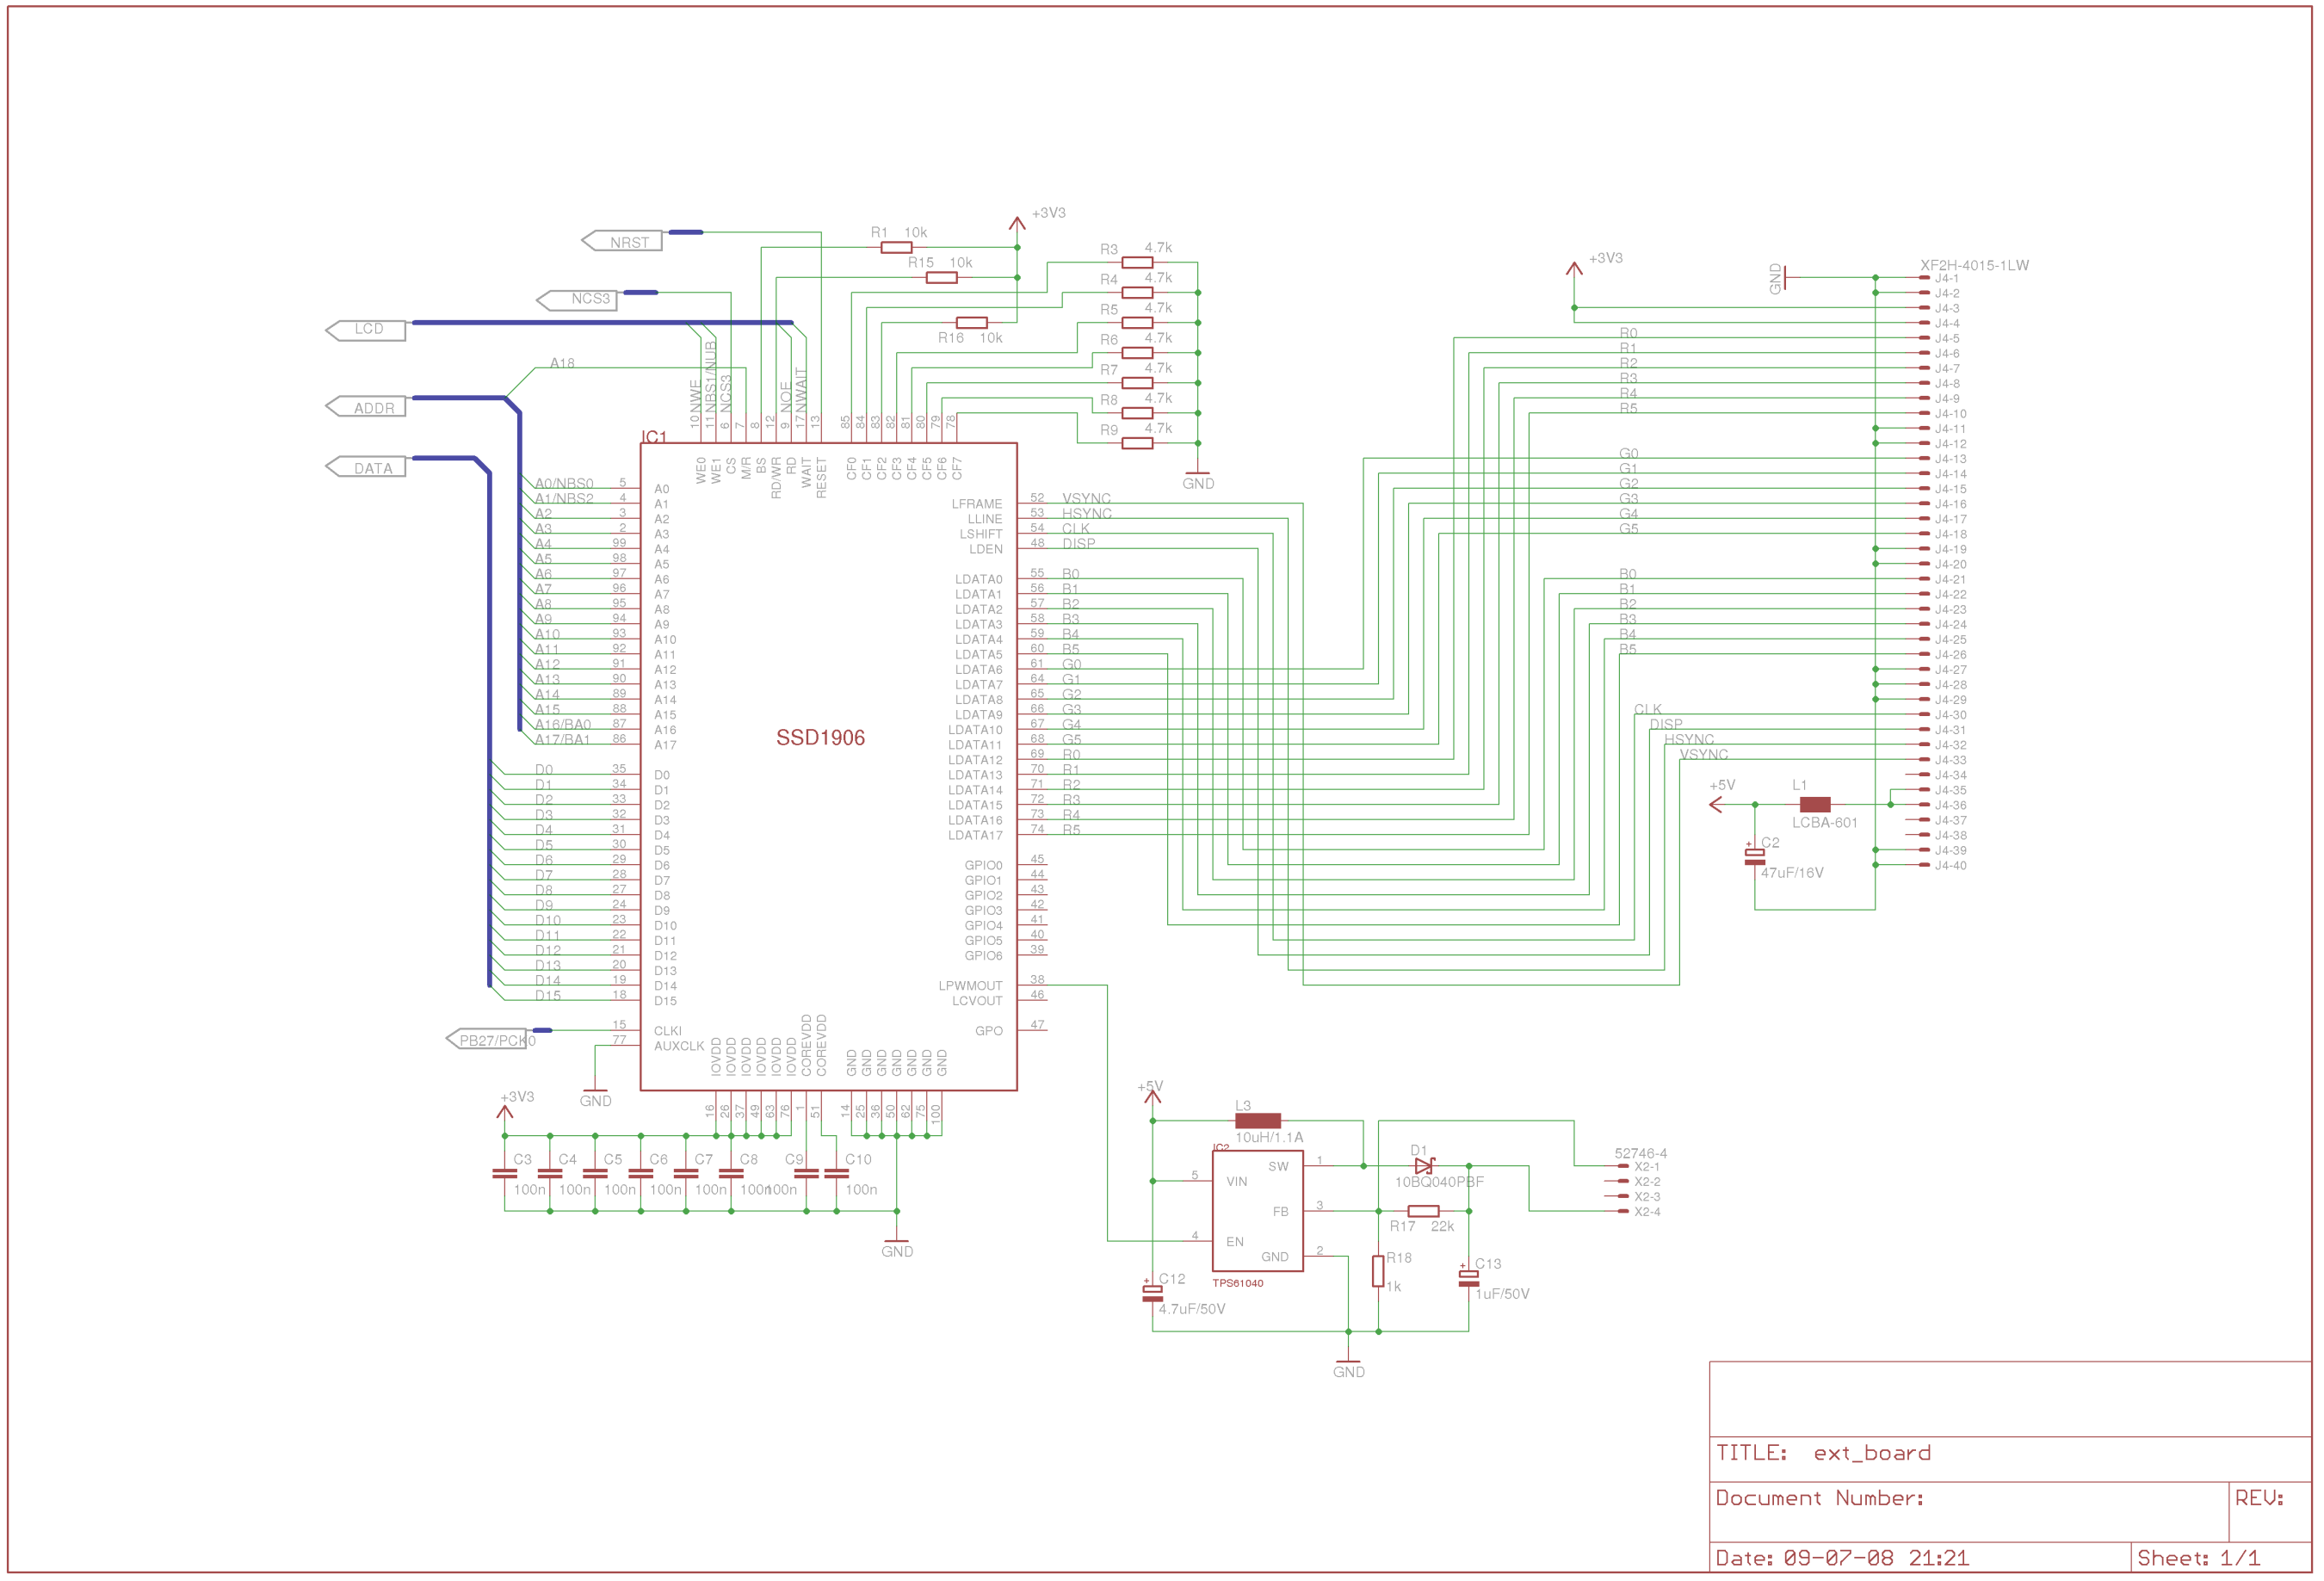
\includegraphics[scale=1.0,angle=90]{img/ext_sch1.png}
				\caption{Schemat podłączenia wyświetlacza i kontrolera LCD}
			\end{center}
		\end{figure}
		
		\begin{figure}[]
			\begin{center}
				\label{fig:ext_sch_rest}
				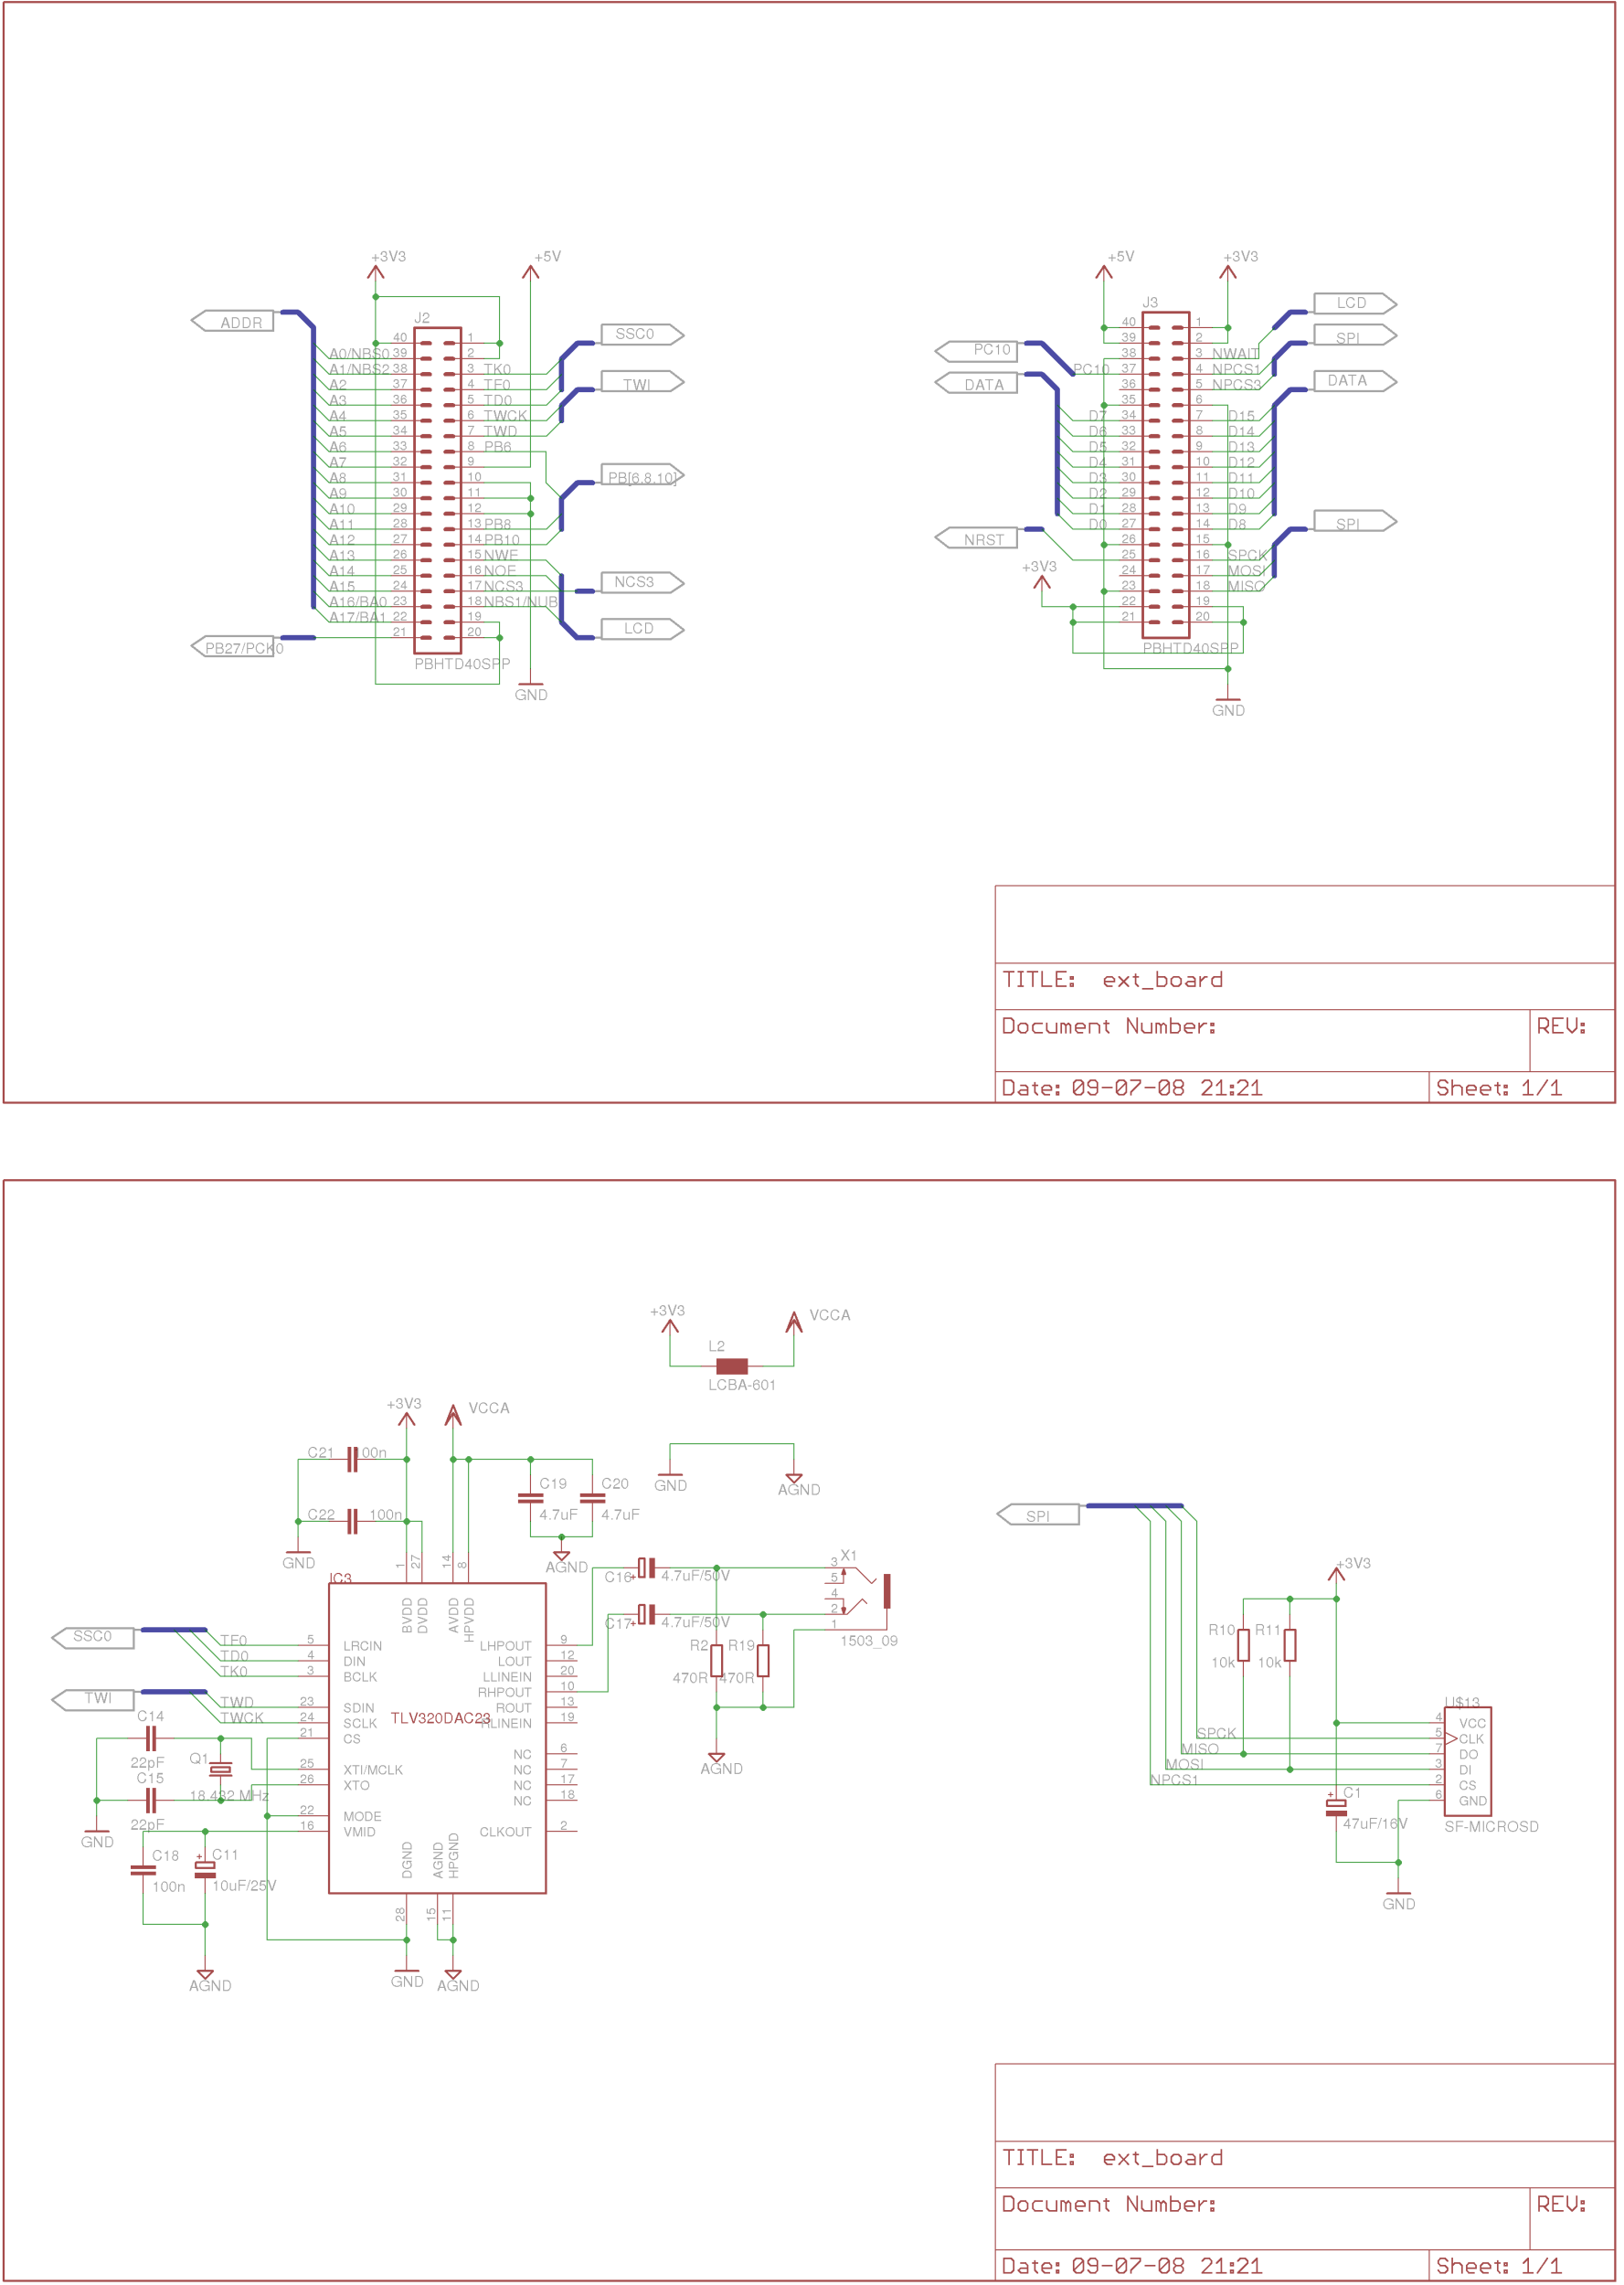
\includegraphics[scale=1.0]{img/ext_sch2.png}
				\caption{Schemat podłączenia dodatkowych elementów rozszerzających możliwości projektu}
			\end{center}
		\end{figure}
				
		\begin{figure}[]
			\begin{center}
				\label{fig:main_brd}
				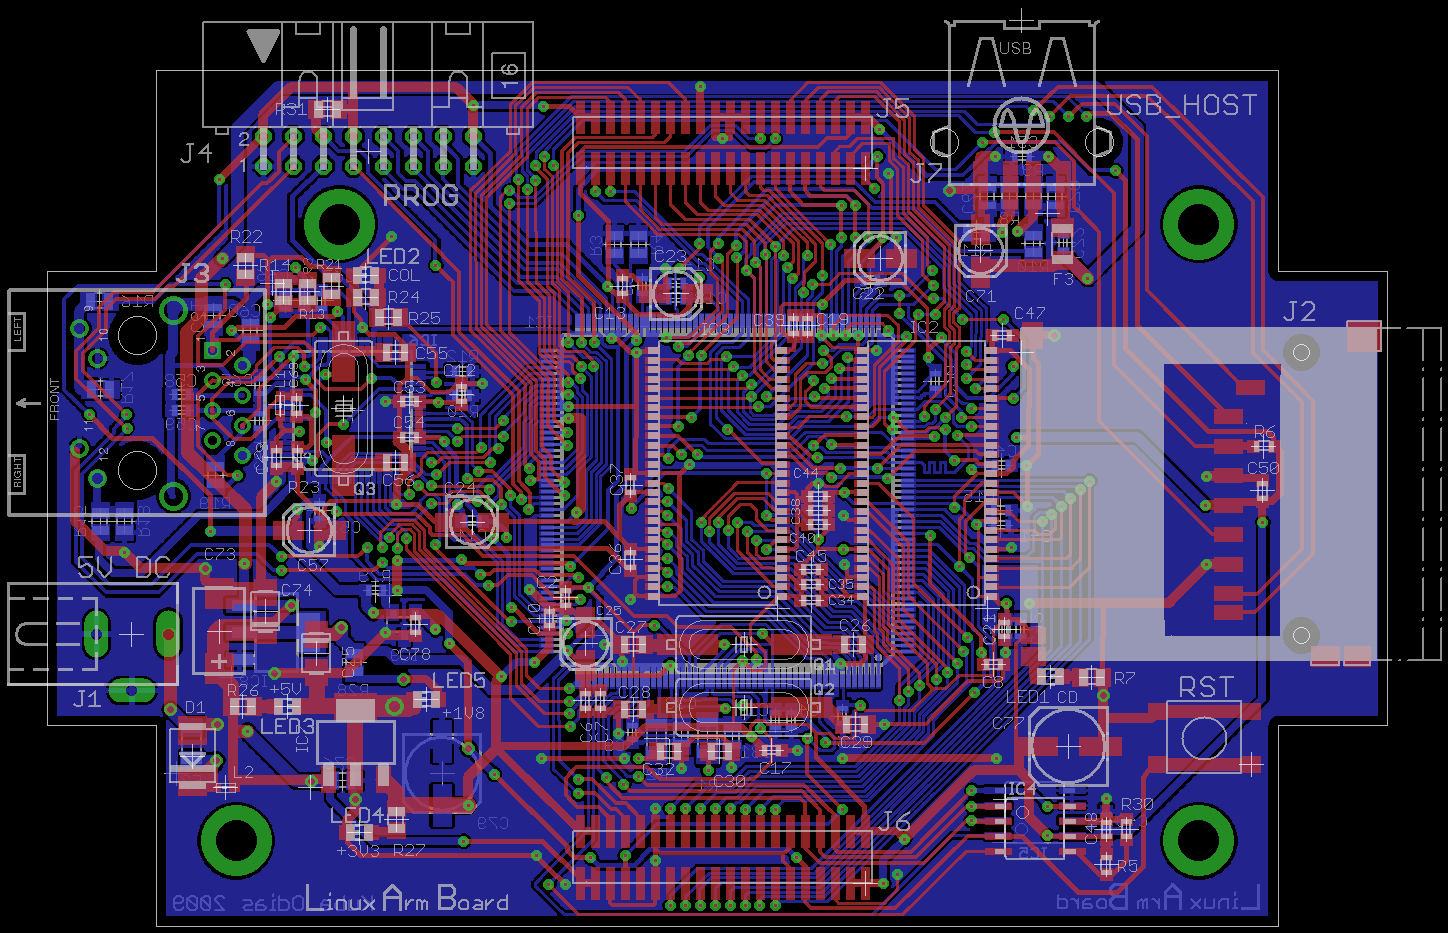
\includegraphics[scale=1.25]{img/main_brd.png}
				\caption{Plik .brd programu Eagle dla głównej płytki}
			\end{center}
		\end{figure}
		
		\begin{figure}[]
			\begin{center}
				\label{fig:ext_brd}
				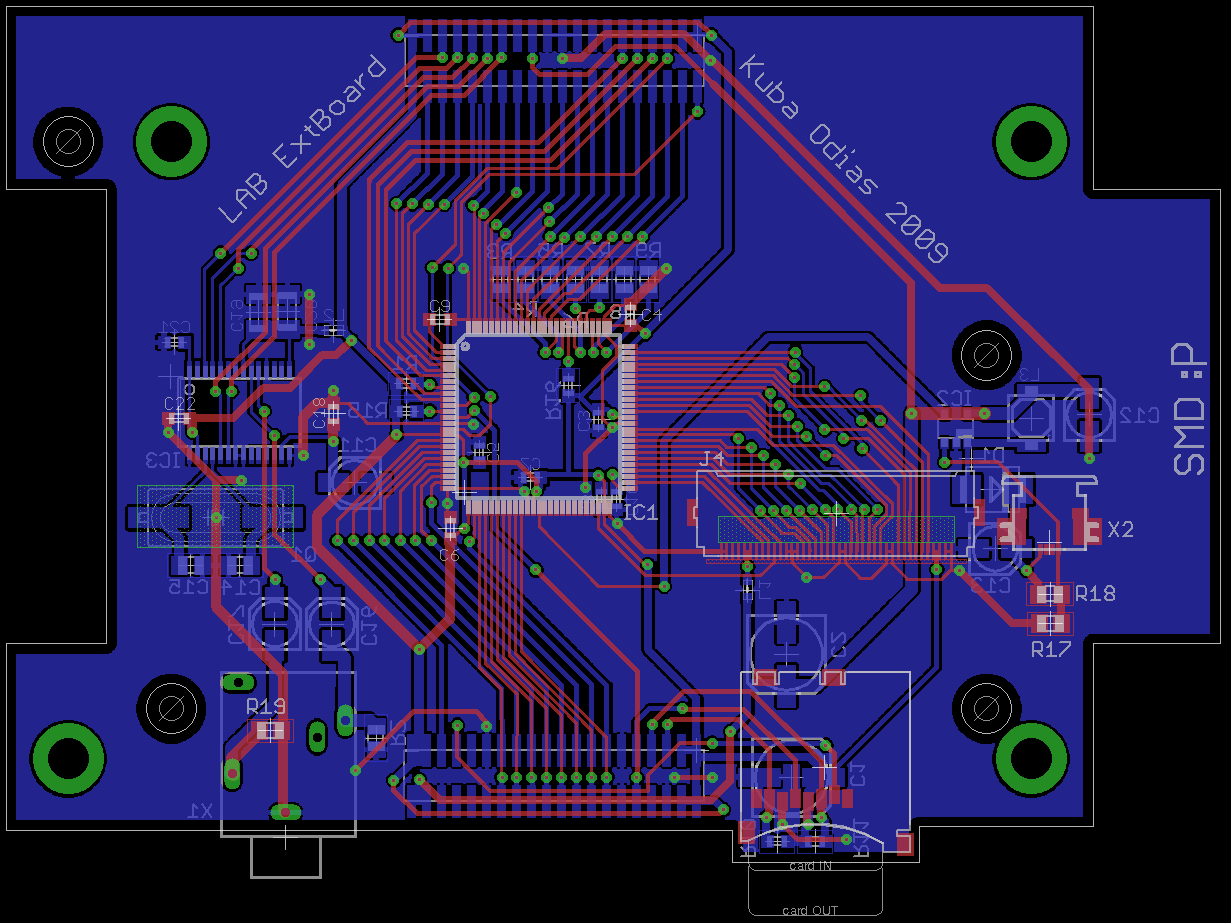
\includegraphics[scale=1.25]{img/ext_brd.png}
				\caption{Plik .brd programu Eagle dla dodatkowej płytki}
			\end{center}
		\end{figure}
		
		\newpage
		\makebox{}
		\newpage
		
		\begin{figure}[h!]
			\begin{center}
				\subfigure[Górna strona]{\label{fig:pcb1-top}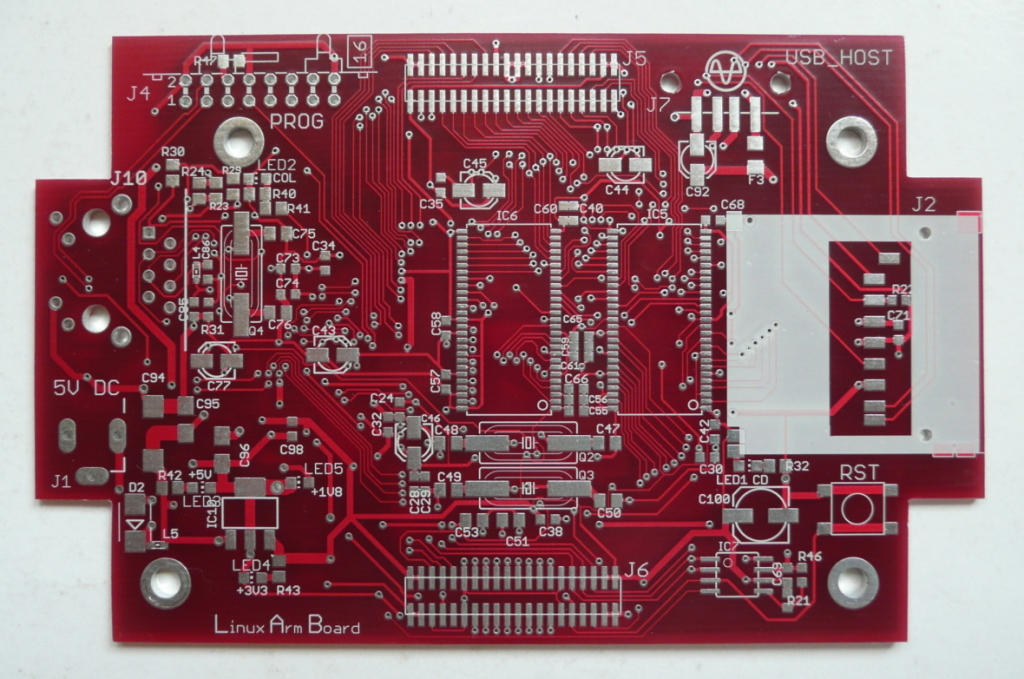
\includegraphics[scale=0.25,angle=90]{img/pcb1_top.jpg}}
				\hspace{20pt}
				\subfigure[Górna strona z przylutowanymi elementami]{\label{fig:pcb1-ready-top}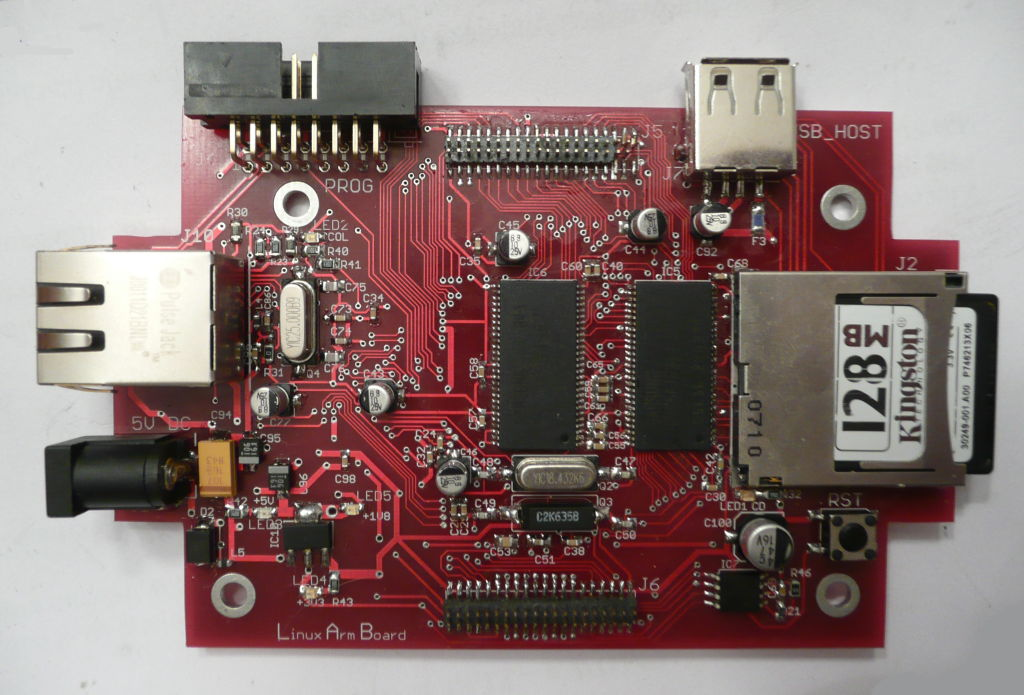
\includegraphics[scale=0.25,angle=90]{img/pcb1_ready_top.jpg}}\\
				\vspace{20pt}
				\subfigure[Dolna strona]{\label{fig:pcb1-bottom}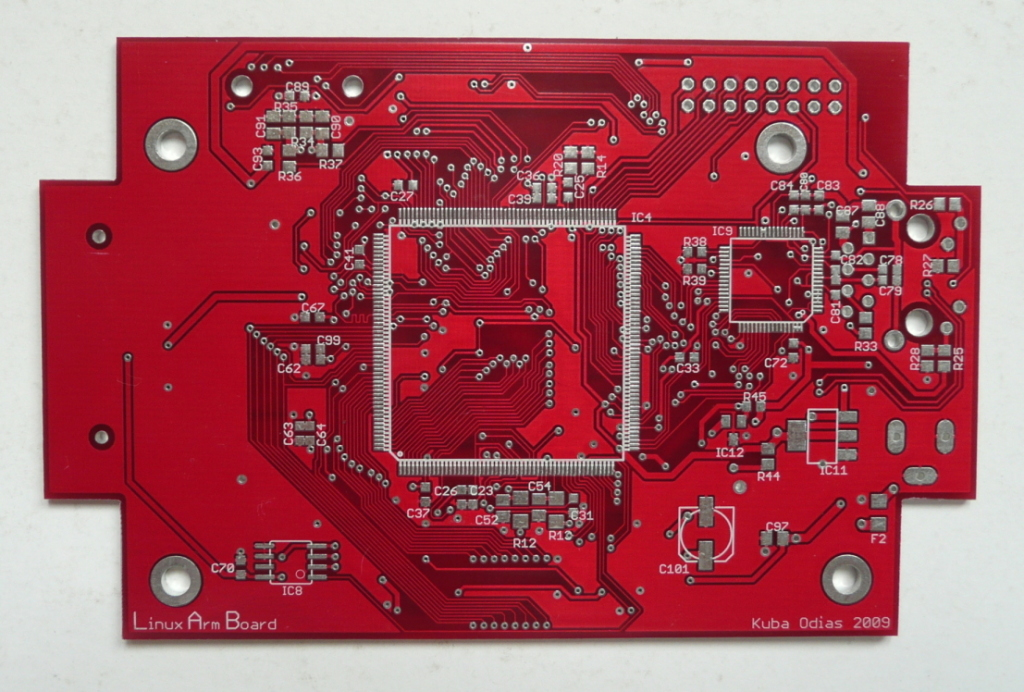
\includegraphics[scale=0.25,angle=90]{img/pcb1_bottom.jpg}}
				\hspace{20pt}
				\subfigure[Dolna strona z przylutowanymi elementami]{\label{fig:pcb1-ready-bottom}\includegraphics[scale=0.25,angle=90]{img/pcb1_ready_bottom.jpg}}
			\end{center}
			\caption{Główna płytka drukowana}
			\label{fig:pcb1}
		\end{figure}
		
		\newpage
		\makebox{}
		\newpage
		
		\begin{figure}[h!]
			\begin{center}
				\subfigure[Górna strona]{\label{fig:pcb2-top}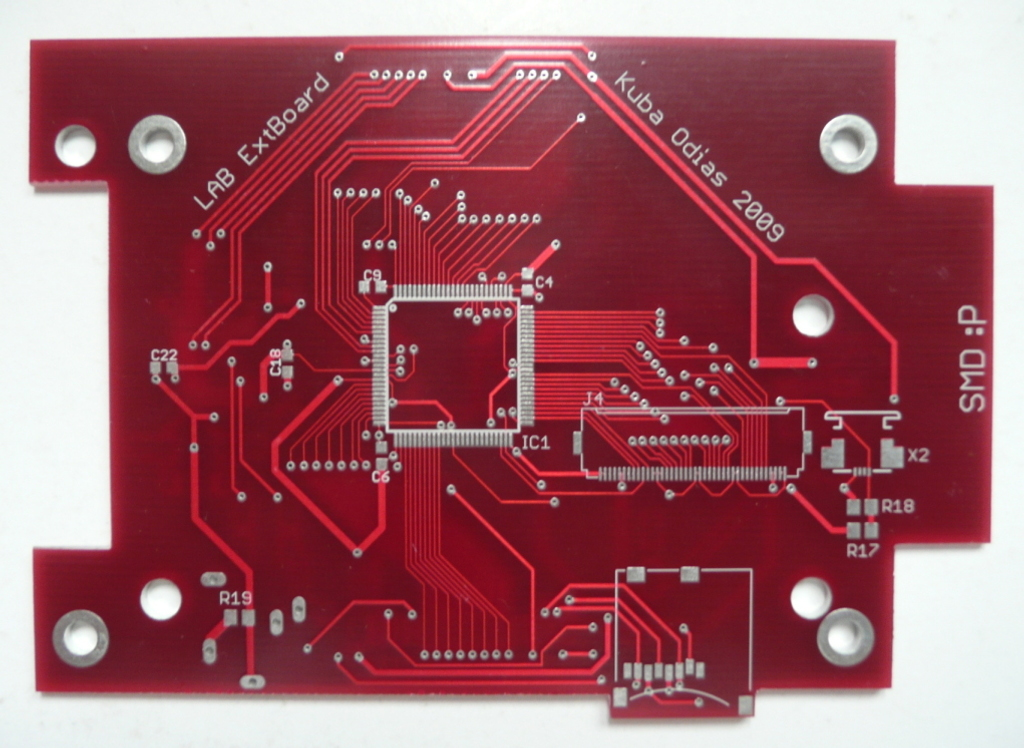
\includegraphics[scale=0.25,angle=90]{img/pcb2_top.jpg}}
				\hspace{20pt}
				\subfigure[Górna strona z przylutowanymi elementami]{\label{fig:pcb2-ready-top}\includegraphics[scale=0.25,angle=90]{img/pcb2_ready_top.jpg}}\\
				\vspace{20pt}
				\subfigure[Dolna strona]{\label{fig:pcb2-bottom}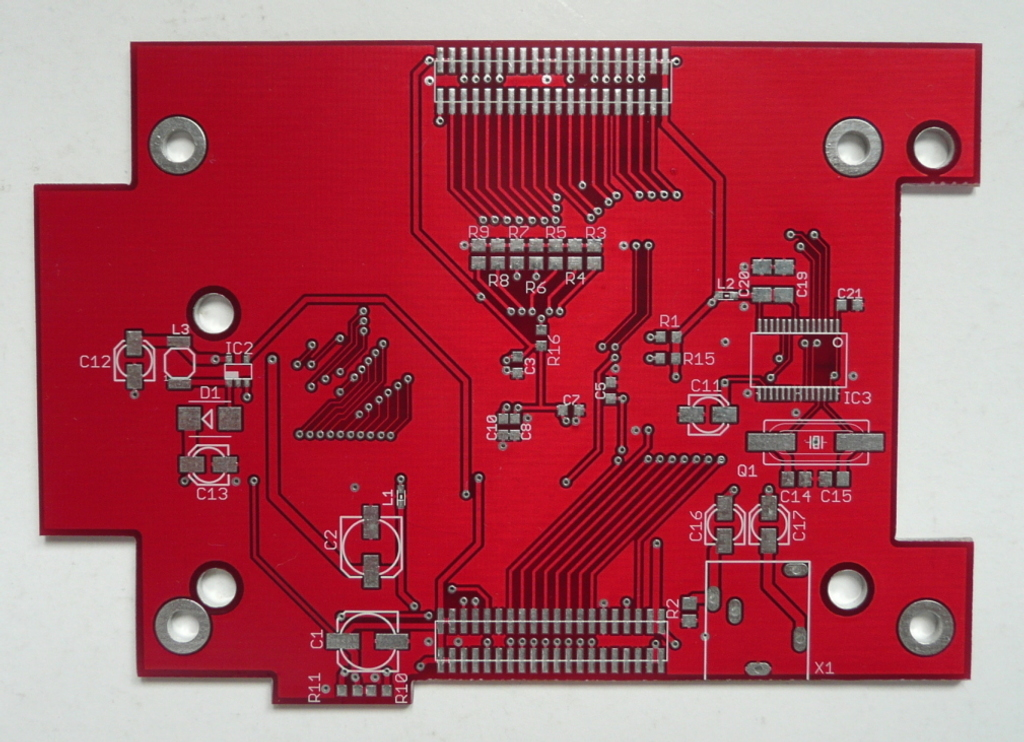
\includegraphics[scale=0.25,angle=90]{img/pcb2_bottom.jpg}}
				\hspace{20pt}
				\subfigure[Dolna strona z przylutowanymi elementami]{\label{fig:pcb2-ready-bottom}\includegraphics[scale=0.25,angle=90]{img/pcb2_ready_bottom.jpg}}
			\end{center}
			\caption{Dodatkowa płytka drukowana}
			\label{fig:pcb2}
		\end{figure}
	
		\newpage
		\makebox{}
		\newpage
		
		\begin{figure}[h!]
			\begin{center}
				\subfigure[Zdjęcie 1]{\label{fig:project-ready1}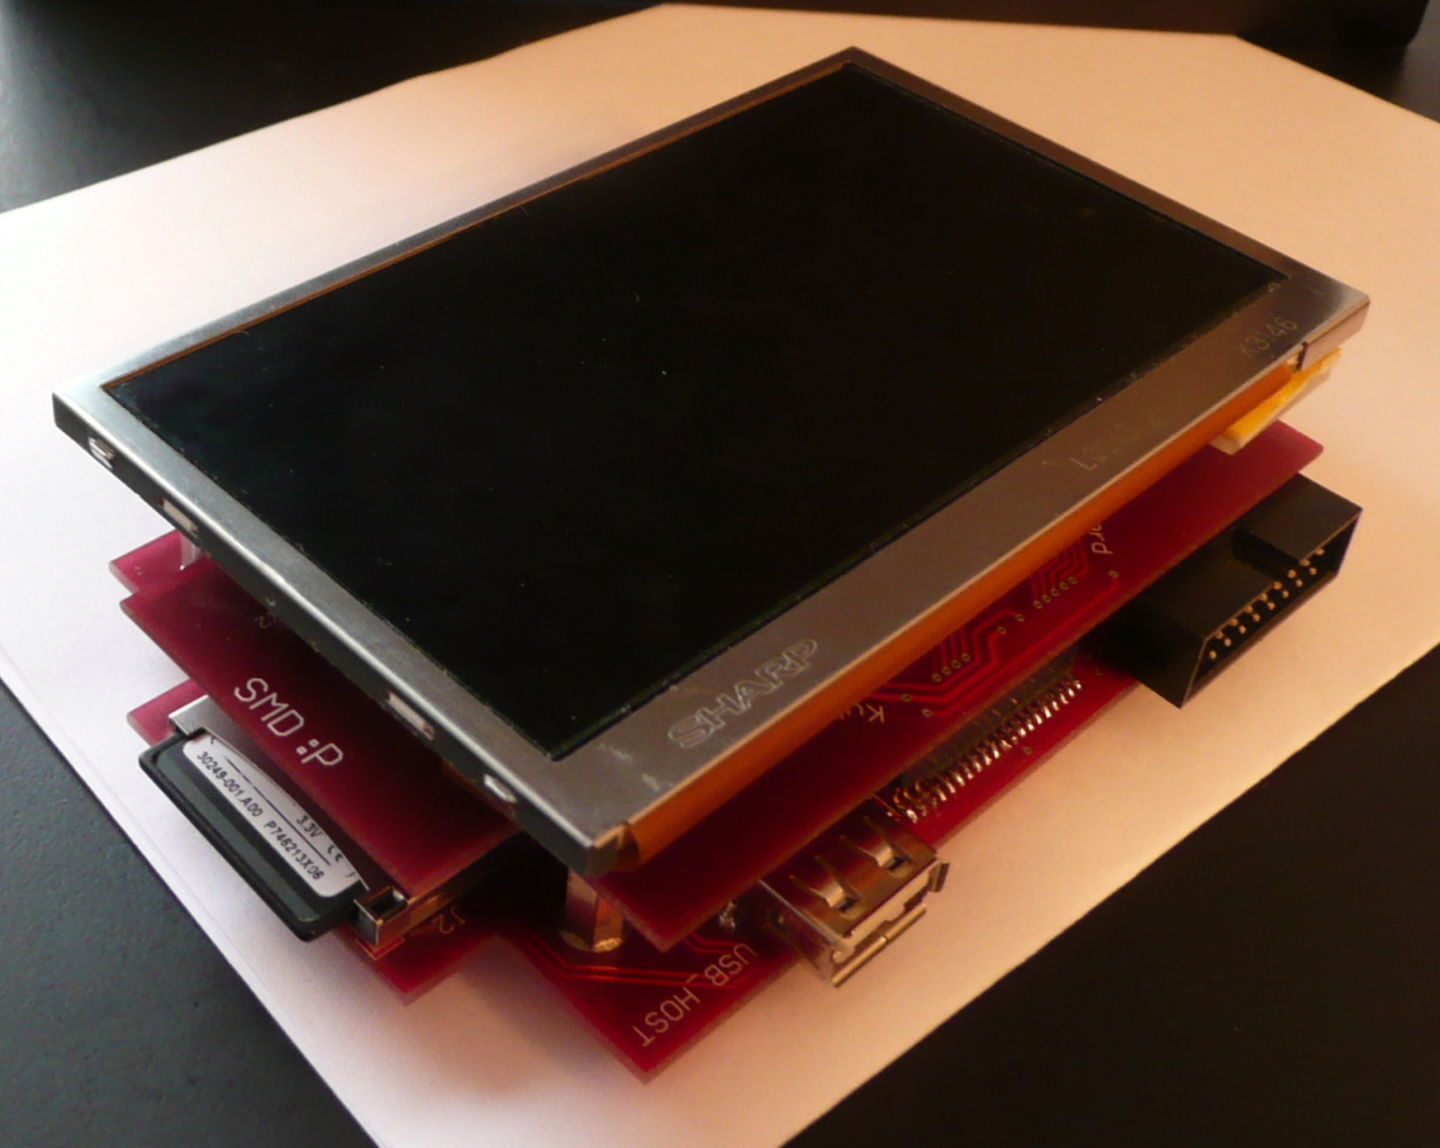
\includegraphics[scale=0.25]{img/project_ready1.jpg}}\\
				\vspace{30pt}
				\subfigure[Zdjęcie 2]{\label{fig:project-ready2}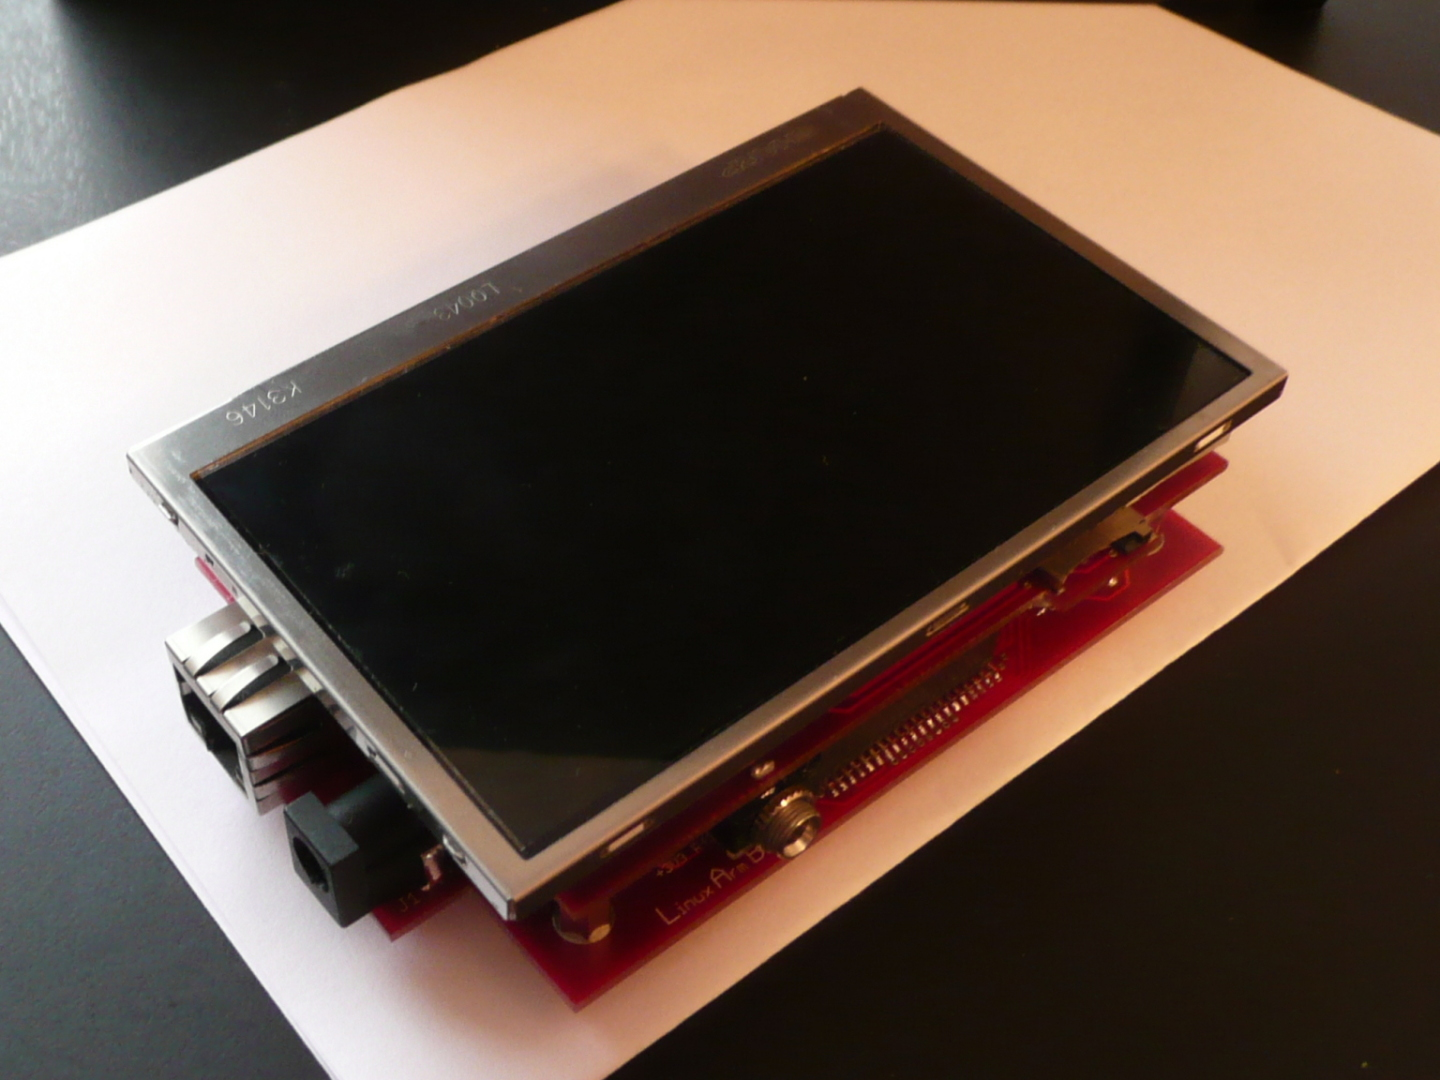
\includegraphics[scale=0.25]{img/project_ready2.jpg}}
			\end{center}
			\caption{Gotowy projekt razem z wyświetlaczem LCD}
			\label{fig:project-ready}
		\end{figure}
		
		\newpage
		\makebox{}
		\newpage
		
		\begin{figure}[h!]
			\begin{center}
				\subfigure[Schemat ideowy programatora wykonany w programie Eagle]{\label{fig:programator_sch}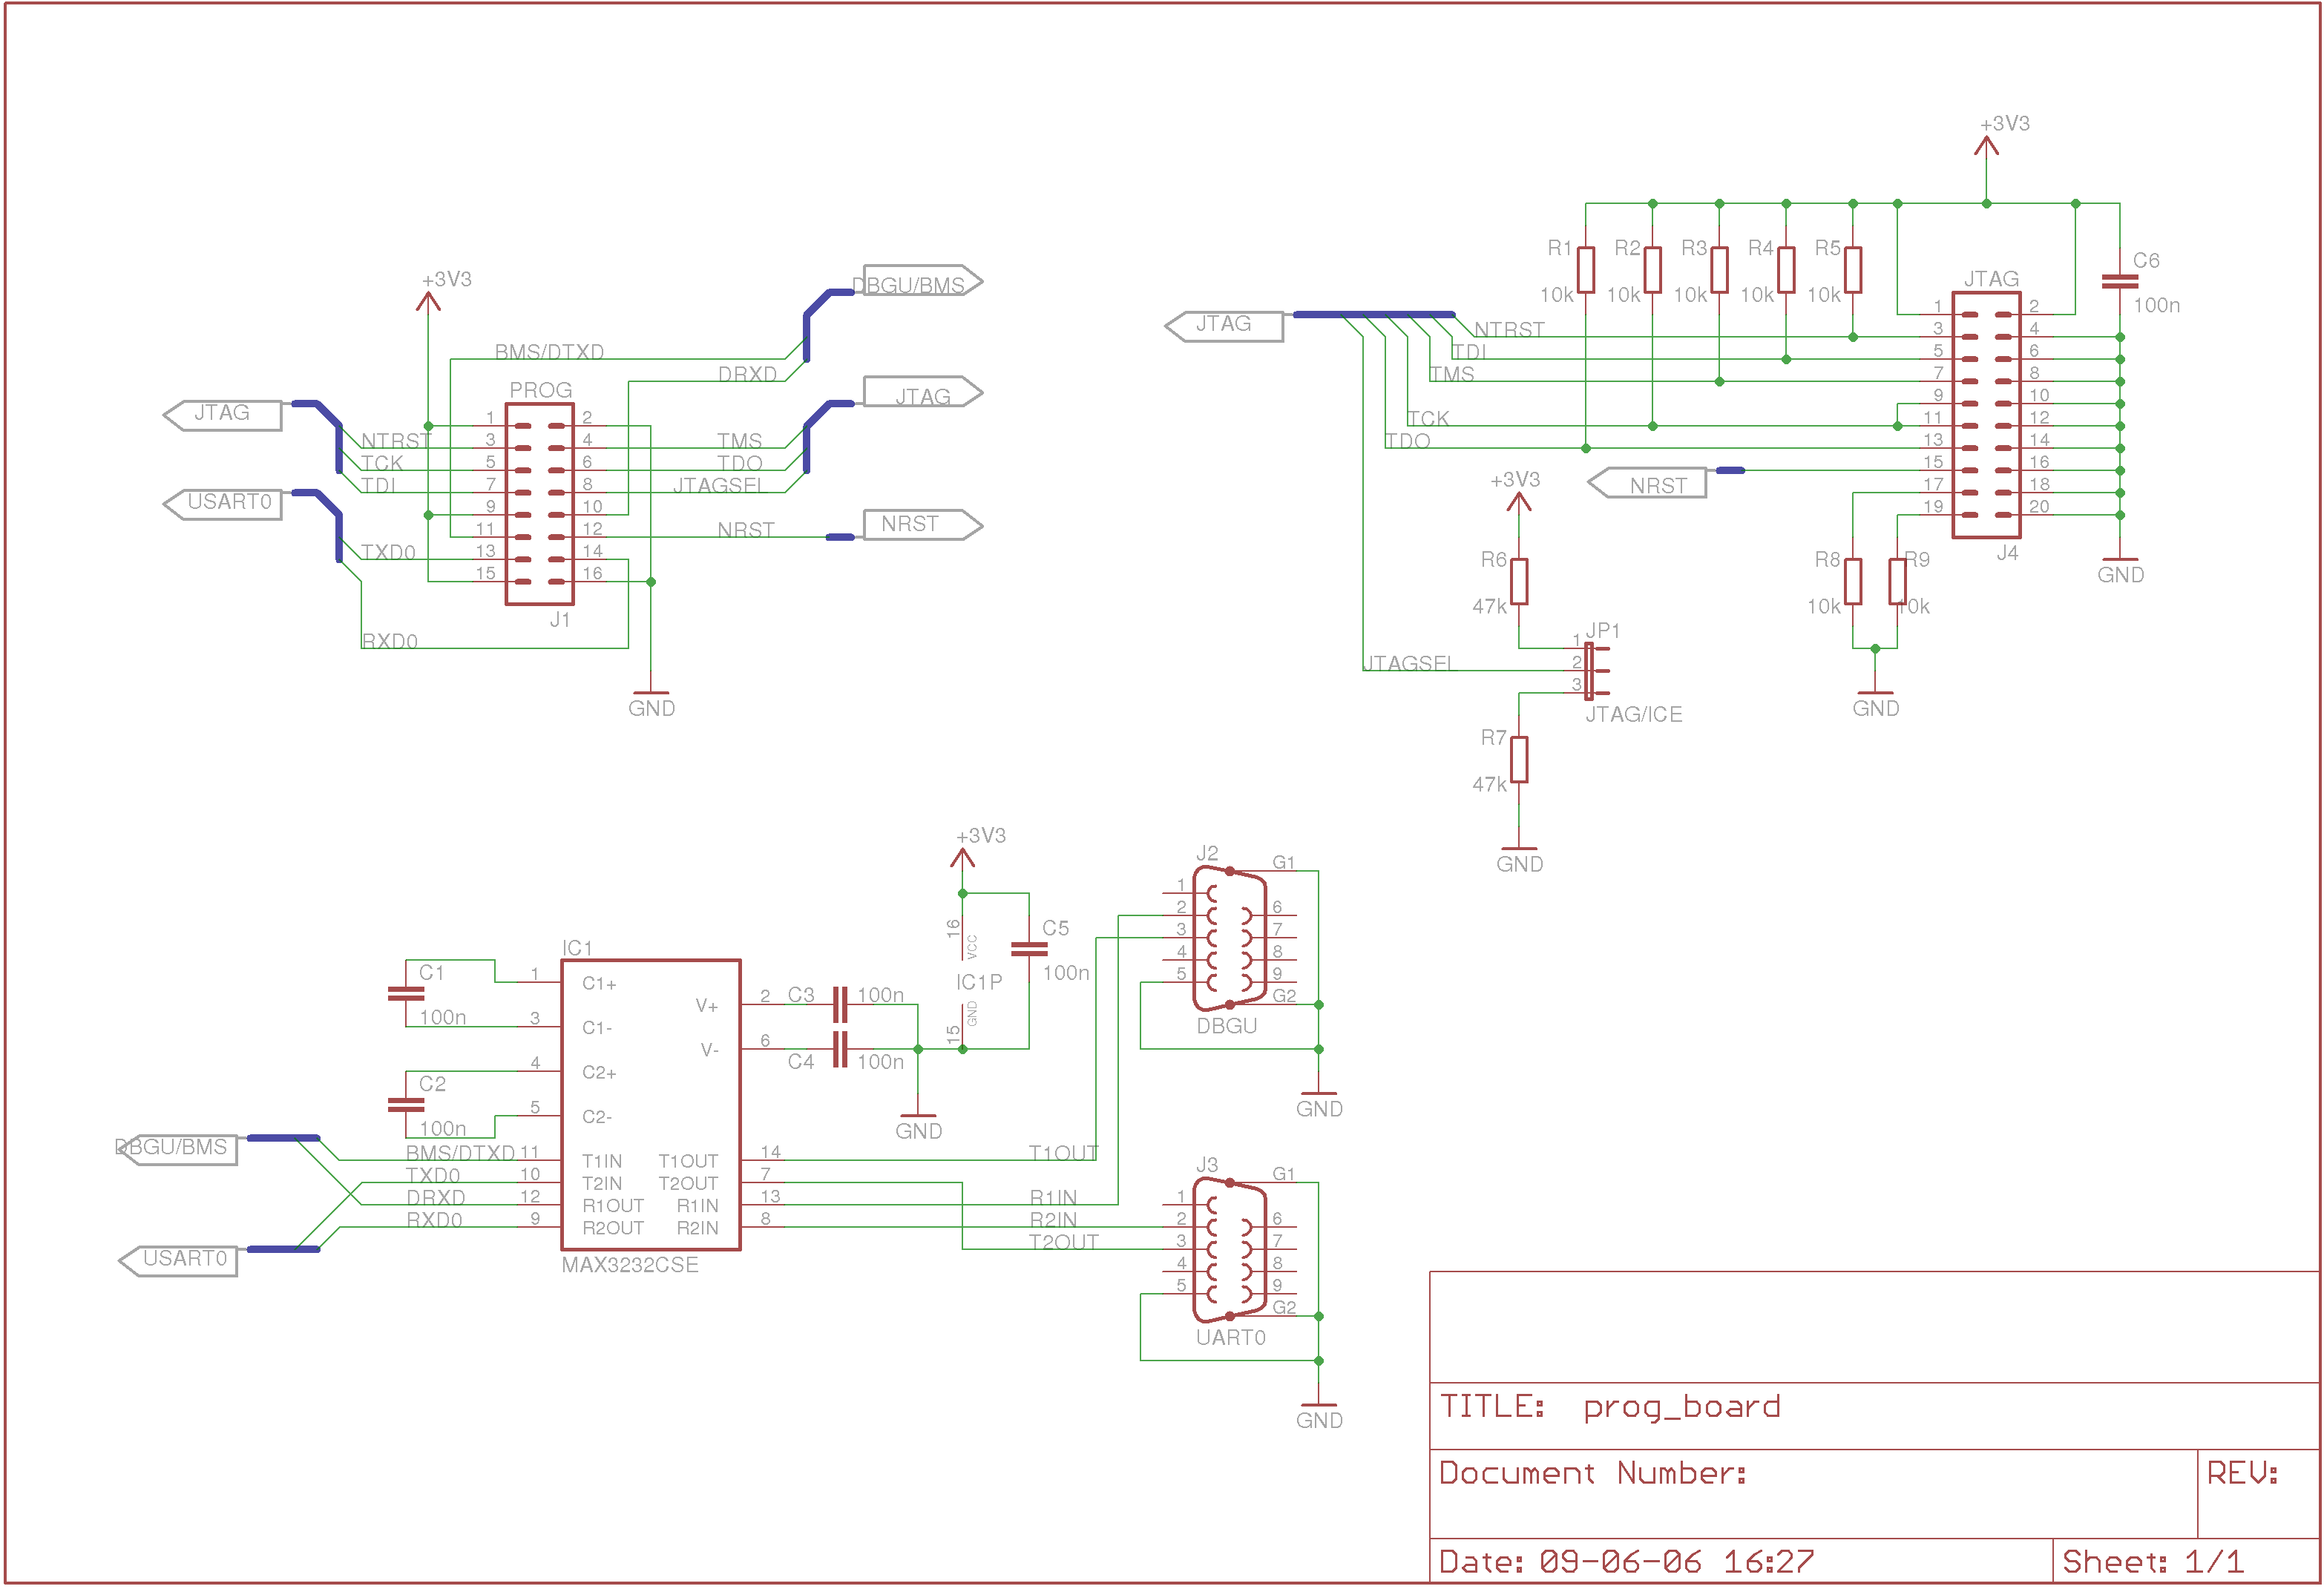
\includegraphics[scale=0.55]{img/programator_sch.png}}\\
				\vspace{40pt}
				\subfigure[Plik .brd programu Eagle dla programaora]{\label{fig:programator_brd}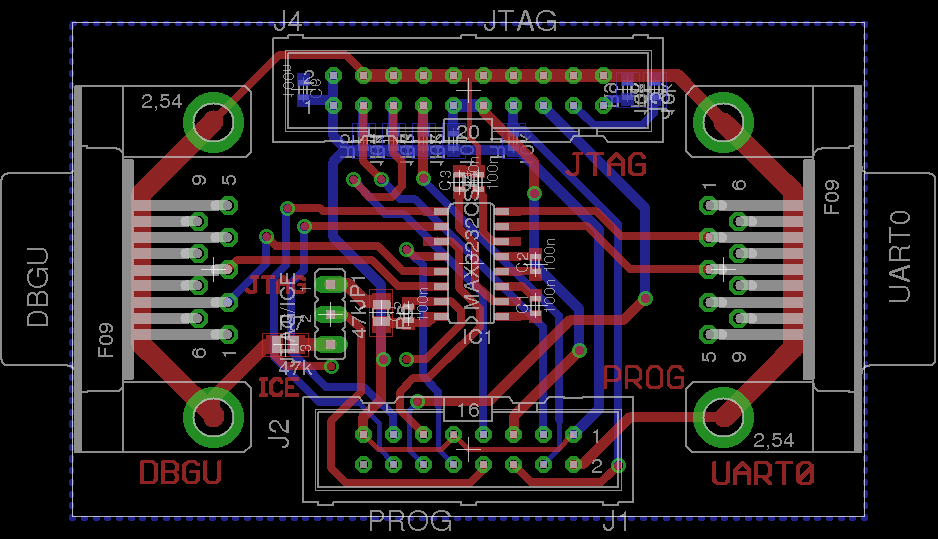
\includegraphics[scale=1.4]{img/programator_brd.png}}
			\end{center}
			\caption{Projekt programatora}
			\label{fig:programator}
		\end{figure}

	
	\chapter{Przykładowe projekty}
	\label{app:przykladowe_projekty}
	\begin{itemize}
		\item \texttt{http://www.atmel.com/dyn/resources/prod\_documents/doc6103.pdf}\\
			Zestaw uruchomieniowy firmy Atmel dla AT91RM9200.\\
			\scriptsize{(strona odwiedzana w dniu 15.08.2009)}
			\normalsize
		\item \texttt{http://blackmesaeast.com.pl/projects/electronics/sarge-single-\\board-computer/}\\
			Projekt autorstwa Grzegorza Rajtara wykorzystujący mikrokontroler AT91RM9200 i kontroler sieciowy STE100P.\\
			\scriptsize{(strona odwiedzana w dniu 15.08.2009)}
			\normalsize
		\item \texttt{http://bryndza.boff.pl/index.php?dz=proj\&id=armputer210}\\
			Projekt autorstwa Lucjana Bryndzy pełniący rolę serwera sieciowego.\\
			\scriptsize{(strona odwiedzana w dniu 15.08.2009)}
			\normalsize
		\item \texttt{http://www.olimex.com/dev/sam9-L9261.html}\\
			Zestaw uruchomieniowy firmy Olimex dla mikroprocesora AT91SAM9261.\\
			\scriptsize{(strona odwiedzana w dniu 15.08.2009)}
			\normalsize
	\end{itemize}
	
\end{document}